Powder Bed Fusion (PBF), like all industrial processes, relies on parameters control that ensures its proper functioning. When a process shows the expected behavior, it's referred to as "in-control process". On the other hand, when the process deviates from the desired behavior, its output becomes unpredictable, and it's referred as "out-of-control" (OOC). When a process is out of control, anomalies and defects can arise in the output. In Section \ref{sec:defects}, we will describe most common defects in PBF processes and their causes. In Section \ref{sec:comelotrovo} we will discuss different approaches for defects detection, while in Section \ref{sec:sensoriniiniini} I will report available sensors used in anomalies detection.  Sections of this chapter are mainly based on \citeauthor{grasso_-process_2017} (2017), \citeauthor{grasso_process_2017} (2017), \citeauthor{mostafaei_defects_2022} (2022) and \citeauthor{wu_additively_2023} (2023). Finally, in Section \ref{sec:hotspot}, we will focus on defects caused by anomalies in the temperature profiles of the building bed, the so called hot spots, the core topic of this thesis.

% Categories of Defect in PBF Processes >>>
\section{Defects Categories and Causes in PBF Processes}
\label{sec:defects}
Defects in PBF processes can be divided into five main classes: porosity defects, residual stresses and cracking, geometric defects and dimensional accuracy, balling and surface defects.
\paragraph{Porosity.} Porosity is a really significant parameters for many metal AM applications, as it strongly impacts on fatigue resistance and crack propagation in the component \cite{edwards_electron_2013}. 
\begin{figure}
    \centering
    \subfloat[\label{fig:poris}]{
        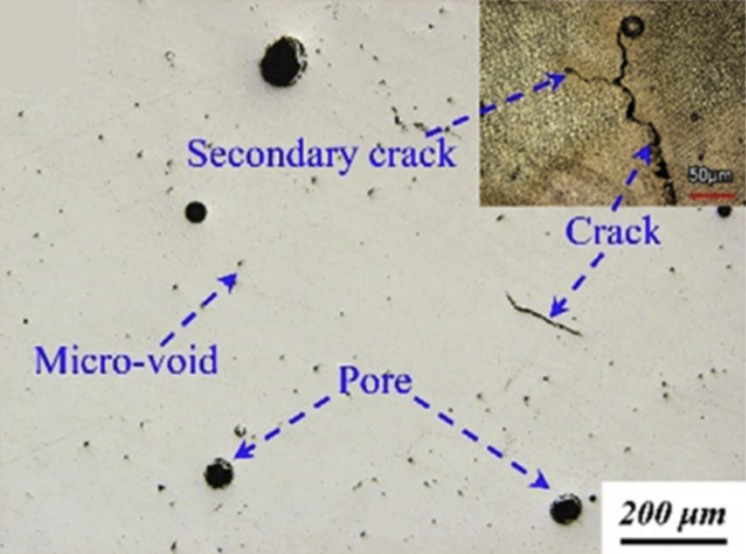
\includegraphics[scale=0.4]{Images/pori e crack.png}
    }
    \qquad
    \subfloat[\label{fig:acircular}]{
        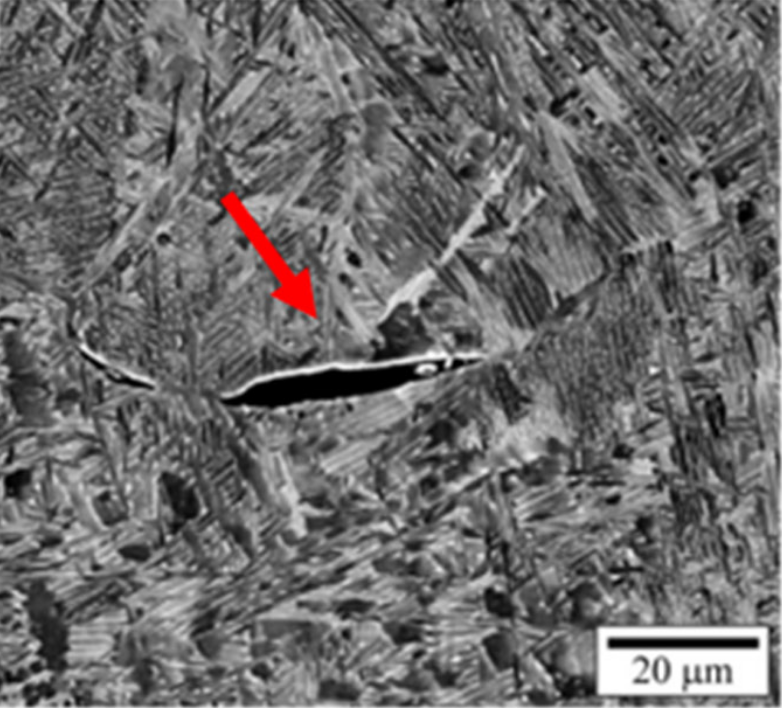
\includegraphics[scale=0.31]{Images/acircular.png}
    }
    \qquad
    \subfloat[\label{fig:delamination}]{
        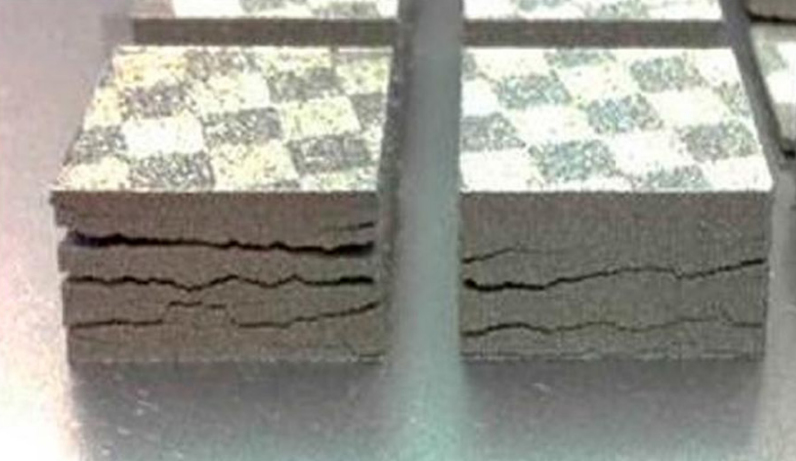
\includegraphics[scale=0.4]{Images/delamination.png}
    }
    \qquad
    \subfloat[\label{fig:balling}]{
        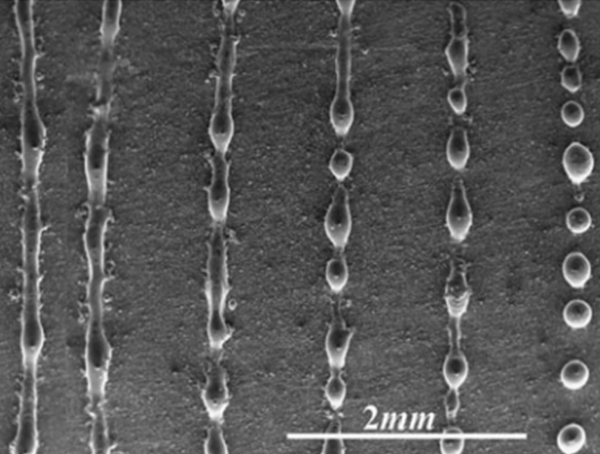
\includegraphics[scale=0.4]{Images/balling.png}
    }
    \caption[Defect examples in PBF.]{Pores, micro-void and cracks in a specimen of FeCrCoMnNi (a) \cite{mostafaei_defects_2022}, an acircular pores on a specimen of Ti–6Al–4V (b) \cite{tammas-williams_xct_2015}, an example of delamination in SLS (c) \cite{sames_metallurgy_2016} and the balling effect in stainless steal powder (d) \cite{li_balling_2012}.}
\end{figure} 
Porosity is characterized by empty spaces within the mass of the fused material. These voids can appear within a layer, between adjacent layers, or on the surface of printed piece. Voids most frequently appear within the layer and can vary in size, form, and distribution. The primary causes for these pores include incomplete fusion in the powder bed (lack of fusion or LOF), keyhole effects, and encapsulated gas. We can also differentiates between round and non-round pores. Some examples of round pores can be seen in Fig. \ref{fig:poris}. The elongated voids observed between layers are labeled as 'acicular pores' and they are recognized by their stretched form and larger size. For example, the acircular pore in Fig. \ref{fig:acircular} has a measure of \SI{20}{\micro\metre}. Pores can either be dispersed throughout the material or primarily situated between the inner patterned area and the outer boundary, known as under-skin pores. Pores can also appear on the exterior surface, where they are typically termed 'surface porosity'.
\paragraph{Residual stresses, cracking and delamination.} In material science, residual stresses are internal tensions that remain in the finished piece also once the printing phase is complete. In PBF, this stresses can arise from two different causes: the thermal gradient mechanism and the cool-down phase of molten top layers \cite{mercelis_residual_2006}. Cracking phenomena occurs as a consequence of a stress relief, when the tensile stress exceeds the ultimate tensile strength of the solid material. When the tension is suddenly released, a secondary crack can generate from the main crack. An example of this phenomenon can be seen in \ref{fig:poris}. On the other hand, delamination happens when cracks originate and propagate between adjacent layers (inter-layer cracking). This happens when the residual stresses exceed the binding linkage between the top layer and the previous one. Most of the times, delamination happens from the partial disconnection of the part from the baseplate \cite{sames_metallurgy_2016}, as in Fig. \ref{fig:delamination}.
\begin{figure}
    \centering
    \subfloat[\label{fig:lackofsupport}]{
        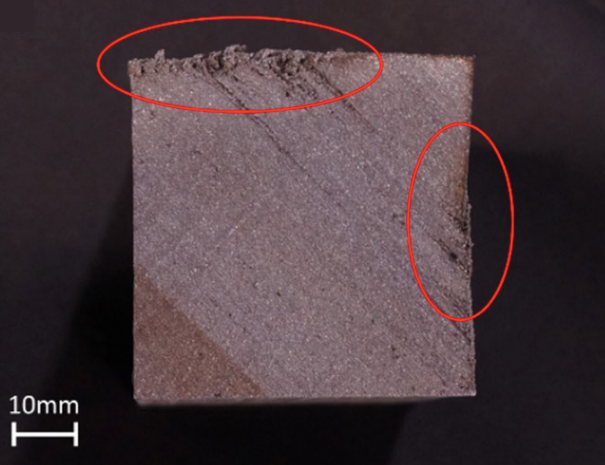
\includegraphics[scale=0.45]{Images/lackofsupport.png}
    }
    \qquad
    \subfloat[\label{fig:oxide}]{
        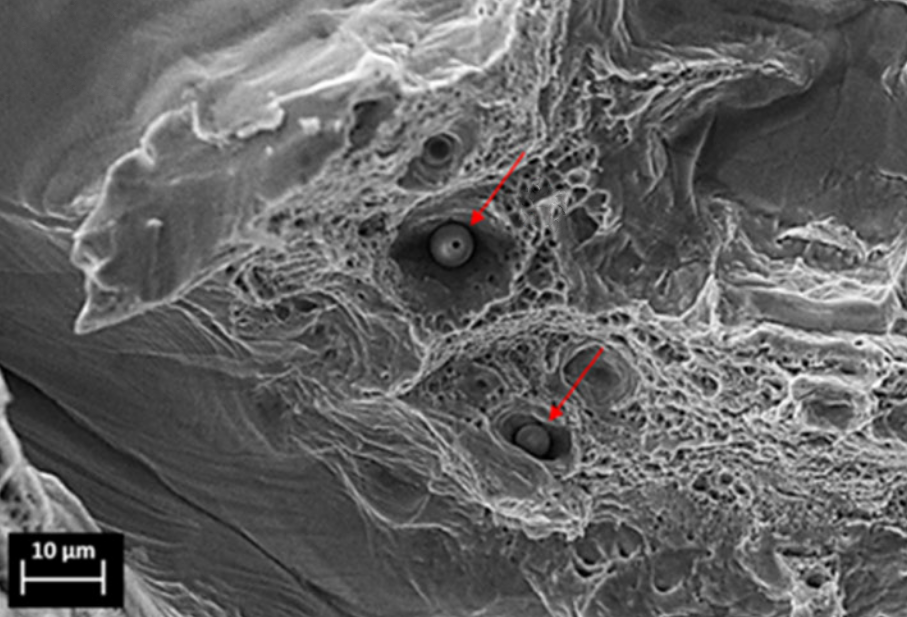
\includegraphics[scale=0.34]{Images/oxide.png}
    }
    \caption[Examples of defect in PBF.]{Example of geometrical errors in SLS caused by a wrong support (a) \cite{grasso_-process_2017}, examples of two local oxide contaminations (b) \cite{casati_microstructure_2016}.}
\end{figure} 
\paragraph{Geometric defects and dimensional accuracy.} Dimensional anomalies in PBF can be categorized into (i) contraction and expansion effects, (ii) warping and curling, (iii) dross formation on bottom-facing surfaces, (iv) super-elevated edges, and (v) additional on-plane geometric distortions. Contraction is among the more common defects, though the opposite effect (i.e., components that are consistently bigger than expected) might arise in certain scenarios. Warping predominantly arises from heat dispersion processes and thermal tensions. In a similar way, curling is a specific bending effect caused by inconsistent thermal growth and component shrinkage, generally tied to disparate contraction rates between the top and underside of overhanging segments. A combination of shrinking and warping effects results in curved outlines for bottom-facing surfaces intended to be flat. Super-elevated edges represent another type of OOC geometrical distortion, featured by elevated ridges of solidified material. These elevated edges not only compromise the final component's integrity but might also be the cause for defects propagation, since they can interfer with recoating blade. Other distortions affect critical features such as thin walls, overhang areas and acute corners. In correspondence of these features, the melt pool is largely surrounded by loose powder, which has a lower conductivity than the solid material. The diminished heat flux yields local over-heating phenomena that may deteriorate the geometric accuracy. This overheated area are called hot spot (HS) and will be discussed in Section \ref{sec:hotspot}.
\paragraph{Balling.} Melt ball formation, a.k.a. balling, occurs when the molten material solidifies into spheres instead of solid layers. This phenomenon is caused by surface tension, which prevents the molten material to spread over previous layer. The result is a rough and bead-shaped surface that produces an irregular layer deposition, with detrimental effects on the density and quality of the final product. \citeauthor{li_balling_2012}(2012) pointed out three main problems when balling happens: (i) increased surface roughness, (ii) large number of pores between the discontinuous metallic balls, and (iii) protruding spheres may interfer with the recoating blade. The latter happens only in presence of a very severe balling. Fig. \ref{fig:balling} show the balling effect on a stainless steal powder.
\paragraph{Surface defects.} In PBF methodologies, as in most of AM processes, the texture of the surface is influenced by the layer-by-layer manufacturing process, and by the existence of surface impurities, inconsistencies, and voids.
\begin{figure}
    \centering
    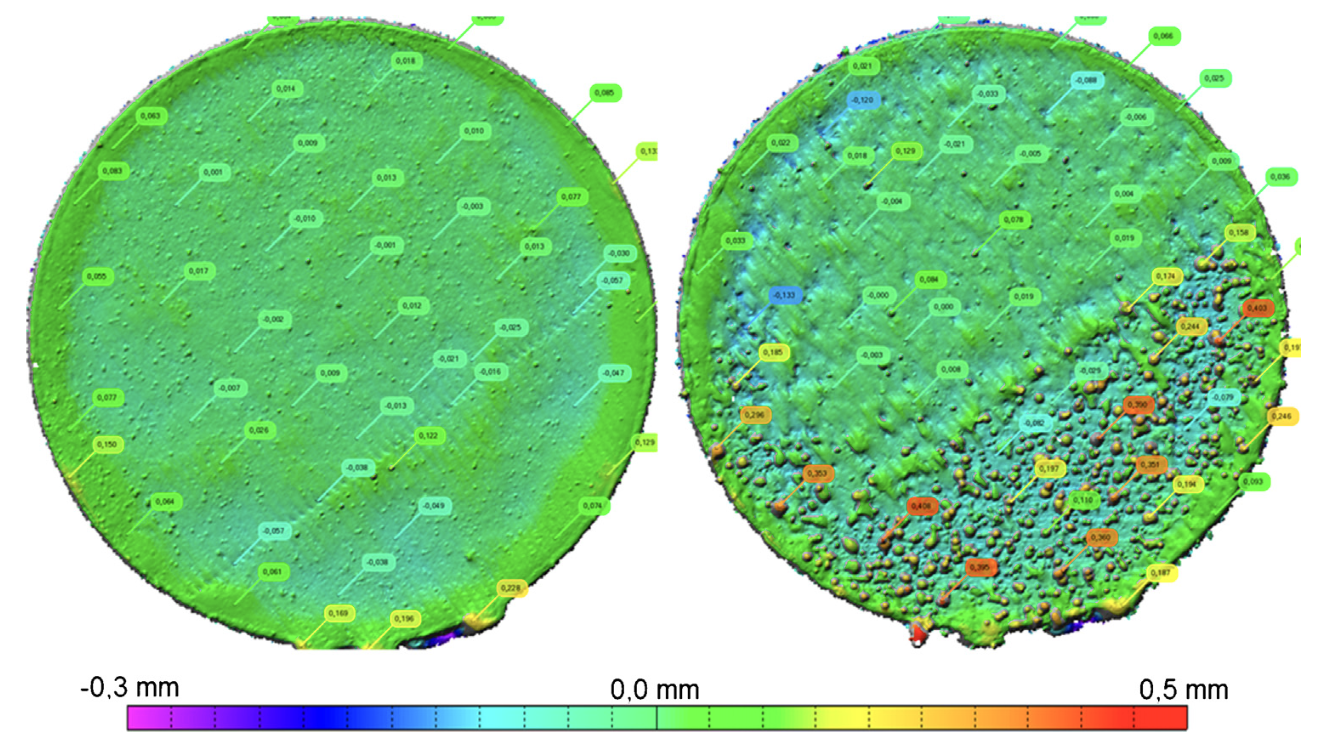
\includegraphics[scale=0.4]{Images/surface.png}
    \caption[Surface roughness in PBF]{Good (left) and poor (right) surface textures measured via confocal microscopy on parts produced either in the presence of good and improper gas flow conditions in L-PBF \cite{ladewig_influence_2016}.}
    \label{fig:surface}
\end{figure}
The surface's texture is determined by processing conditions, the perimeter scanning technique, and the dimensions of powder particles. The orientation of the surface in relation to building direction influences its texture. In particular, downward-facing and upward-facing surfaces are known to have considerably different texture properties. Even though many parts produced via PBF are refined by post-processing operations (like surface polish and thermal procedures), the texture of the surface is of functional importance since it impacts the part's fatigue resilience. Furthermore, for medical lattice structures, the texture of the surface is can help implant's assimilation during bone healing. Fig. \ref{fig:surface} displays instances of optimal (left) and poor (right) surface textures as observed through con-focal microscopy on components made under optimal and improper gas flow situations in L-PBF \cite{ladewig_influence_2016}. Surface imperfections are further increased by the previously mentioned balling phenomenon, leading to less smooth surfaces.
\paragraph{Microstructural inhomogeneities and impurities.} PBF techniques employ extremely localized intense heat inputs over brief durations of beam-material interaction, which in turn markedly influence the part's microstructural composition \cite{thijs_study_2010}. Microstructural discrepancies or non-stable microstructures can potentially impair the mechanical and operational capabilities of the component. Microstructural disparities encompass (i) contaminants, (ii) grain dimension attributes, and (iii) crystallographic orientations \cite{dr_bree_m_sharratt_non-destructive_2015}. Material contaminants consist of inclusions, foreign material adulterations, and oxide layer formations. The existence of non-melted powder particles within voids and/or as isolated powder aggregates has been addressed by several researchers. Fig. \ref{fig:oxide} illustrates a specimen with pronounced defects from oxide formations. These imperfections are believed to be responsible for the premature failure of the specimen and for the reduced strength \cite{casati_microstructure_2016}. In Fig. \ref{fig:microstructuredefect} there are some cracks originated from a microstructure defect.
\begin{figure}
    \centering
    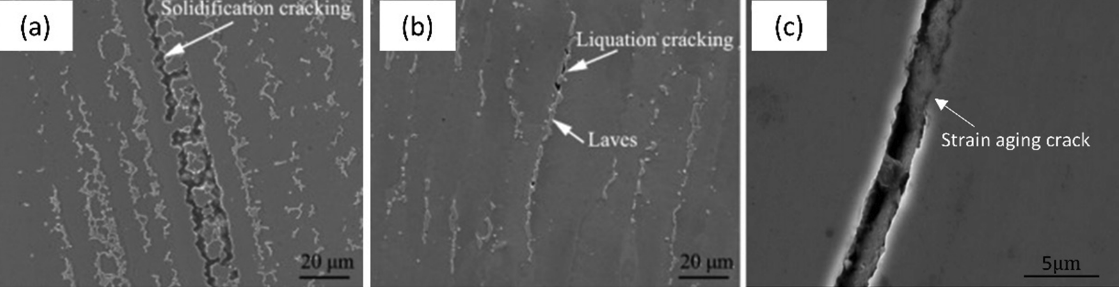
\includegraphics[width=0.7\textwidth]{Images/microstructure.png}
    \caption[Microstructure details.]{Typical microstructure details for AM part delamination and different types of AM cracking: solidification cracking (a); liquation cracking (b); strain aging cracking (c). \cite{mostafaei_defects_2022}.}
    \label{fig:microstructuredefect}
\end{figure}
% <<< End of Categories of Defect in PBF Processes

%%%%%
%%%%%

% >>> Defects Monitoring Methods
\section{Defects Monitoring Methods}
\label{sec:comelotrovo}
In last years, thanks to advancements in both computational power available at lower cost and rising technology of sensors, quality control has evolved into an increasingly complex and sophisticated process. This is particularly evident in AM (Additive Manufacturing), where we can employ the layer-wise production logic to gather vast amounts of data with remarkable granularity. The aim of this section is to outline the various approaches to quality control, providing a terminology framework as established in \citeauthor{richard_leach_integrated_2020} (2020) and in \citeauthor{grasso_-situ_2021} (2021).

\begin{figure}[H]
    \centering
    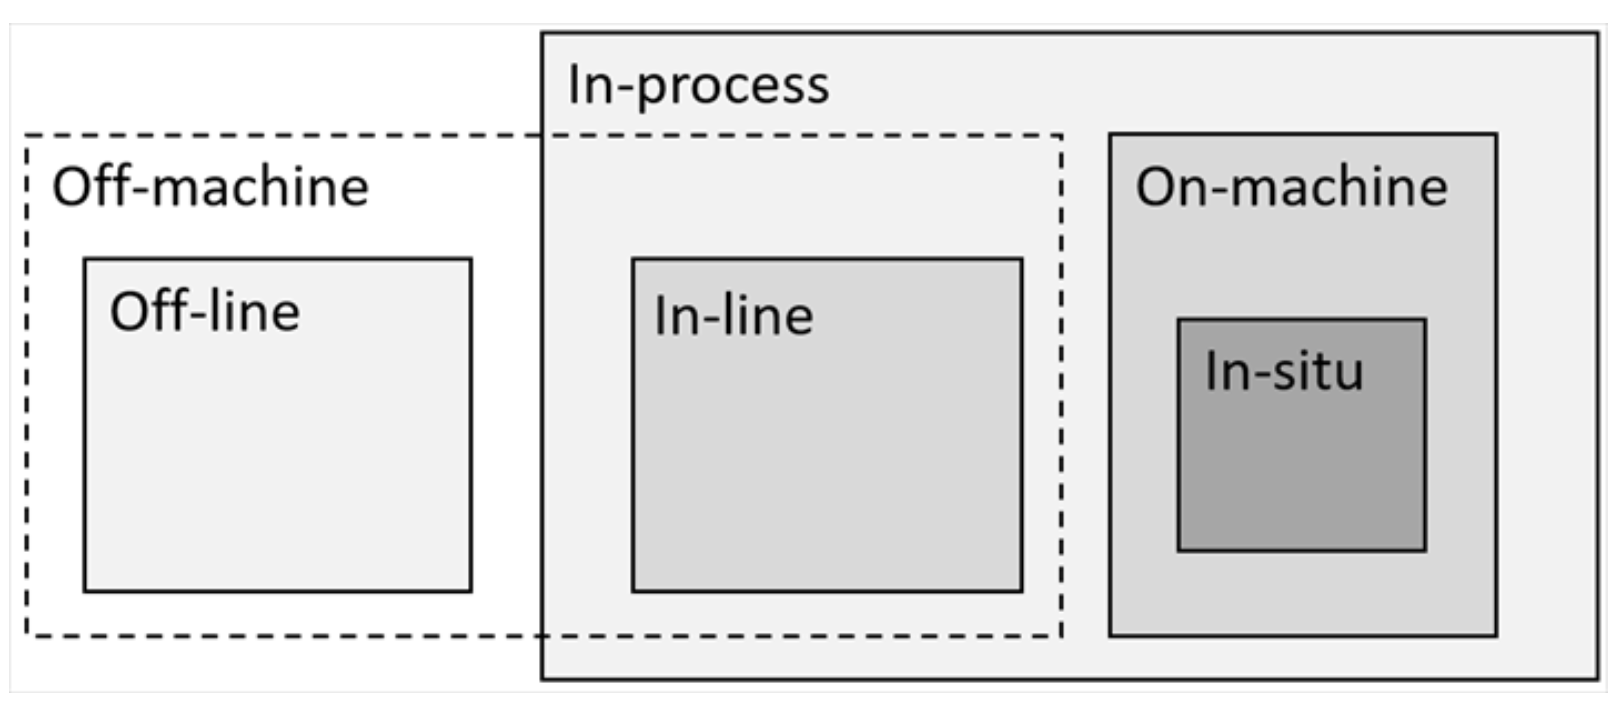
\includegraphics[width=0.6\textwidth]{Images/dovevai.png}
    \caption[Measurement and monitoring techniques.]{Graphical representation of different terms associated with measurement and monitoring techniques \cite{richard_leach_integrated_2020}.}
    \label{fig:dovevai}
\end{figure}
\emph{In-process} methods involve the measurements of any data during the process or between consecutive production phases within the same manufacturing chain. These measurements are syncronized with the different stages of the manufacturing process, thus allowing monitoring it in a synergistic way. When in-process measurements are executed immediately before, after, or amidst manufacturing points, they're called \emph{"in-line"} measurements. These are measured on distinct measurement systems along the standard production line, where manufacturing is not occurring. Consequently, they fall under 'off-machine' measurements. \emph{off-machine} measurements are taken outside the machine where the manufacturing process occurs. On the other hand, if measurements taken during the process use sensors mounted on the production machine, they're labeled \emph{'on-machine'} measurements. Those that principally document data directly from the manufacturing site are called "in-situ" measurements. In AM processes, \emph{in-situ} predominantly denotes sensing and surveillance techniques aiming to capture details about process stability and product quality during the manufacturing process. Data collected from this last method are particularly significant as they are gathered very close to the final product, thus carrying a lot of information. Conversely, when the metrics aren't "in-process", they're labeled as \emph{"off-line"} or \emph{"ex-situ"}. They're categorized as off-machine measurements since they're usually executed outside the core manufacturing setup, perhaps at a separate factory measurement station or a lab. Within the domain of in-situ measurements, there is a small difference between 'in-situ measurement' and 'in-situ monitoring'. The former implies the capability of in-situ sensors to gauge aspects, aiming to understand the process or assess the product's quality attributes during production. The latter alludes to the real-time identification of discrepancies, abnormalities, and unregulated process conditions potentially inducing product flaws, often requiring the establishment of an alert system or classification algorithm.  Furthermore, considering "in-situ" measurements, depending on measured process signature, we can distinguish five different levels of monitoring \cite{grasso_-situ_2021, grasso_process_2017}. These levels are referred to "observable signatures" only, i.e. measurable quantity, while the "derived signatures", i.e. quantitis estimated via process modelling, are included in the process modelling literature. Let's delve into measurements levels for observable signatures, which are summarized in Fig. \ref{fig:levels}.
\begin{figure}
    \centering
    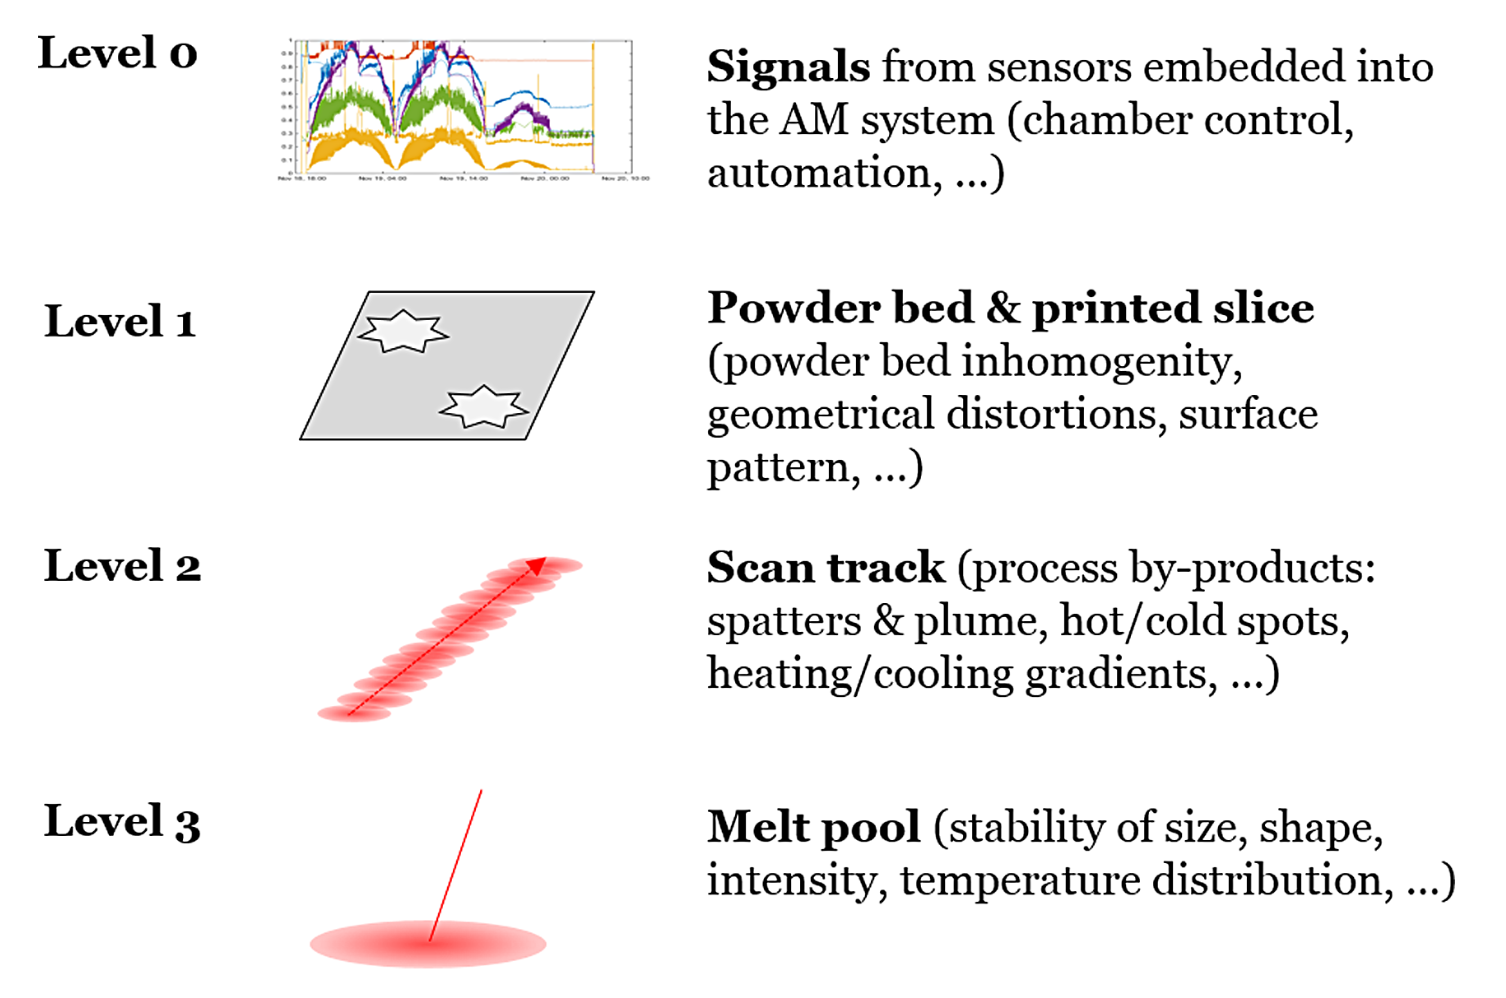
\includegraphics[width=0.8\textwidth]{Images/Level Measurement.png}
    \caption[In-situ measurement levels.]{Four in-situ measurement levels applicable to PBF processes \cite{leach_-machine_2020}.}
    \label{fig:levels}
\end{figure}

\begin{itemize}
    \item \textbf{Level 0:} in this level we use all the signals that can be measured using embedded sensor to detect anomalies and unstable processes state. These sensors usually are employed by printers control unit to keep the machine state and the machine chamber environment under control. Indeed, the main advantage of Level 0 observation is the possibility of monitoring the process without the need for external or additional sensors, especially in EBM printers, where many signals are often already available. However, this signals are often distant from the actual process dynamics, also in terms of “time distance”. Some examples of these signals are chamber pressure, ambient temperature and inert gas flow;
    \item \textbf{Level 1:} this level involves measurements gathered once (or more than once) per layer of the entire build area. We are interested in both the homogeneity of the powder bed and the geometrical and dimensional feature of the printed slice, and in general all the anomalies that can be captured by using a general static 2-d view of the printing plane;
    \item \textbf{Level 2:} this level includes quantities that are representative of the process quality and stability while the beam scans the tracks within the print area. Usually, these quantities can be measured with a temporal resolution higher than the layer-wise resolution in previous level, since we can rely on sensors with really high sampling rates (some cameras can use up to 10,000 fps). It is also higher than the sampling frequency of embedded sensors;
    \item \textbf{Level 3:} this level process signature are the ones with the highest granularity possible in PBF system, i.e. the melt pool. The melt pool is known to be a primary feature of interest in any process that involves a beam-material interaction aimed at achieving a local fusion of the material, since it highly impacts the quality of the part and stability of the process. Some examples of process signatures are the melt-pool size, its shape and the temperature intensity/profile of the melt pool itself;
    \item \textbf{Level 4:} this level regards the capability of gathering information about phenomena occurring under the currently processed layer. These measurements can be obtained with ad-hoc prototype machine configurations that enable transverse x-ray imaging, but also ultrasound and acoustic emissions caused by the release of elastic energy and plastic deformation of solidified layers. The research stream from which this measurement level originated is relatively recent, indeed it is not included in Fig. \ref{fig:levels}.
\end{itemize}
% <<< End of Defect Monitoring Methods

%%%%%
%%%%%

% >>> Sensors for anomalies detection
\section{Sensors for Anomalies Detection}
\label{sec:sensoriniiniini}
Each level described in Section \ref{sec:comelotrovo} involves different sensor tipologies. In this section I will provide a description of the most widely used sensors in in-situ proccess monitoring and measurement in AM. 

In \emph{level ~0}, we can use embedded sensors integrated within the printer, the same sensors that the printing control unit uses to adjust printing parameters. This is particularly suitable in EB-PBF applications, since there are many embedded system to exploit. Embedded sensor signals in EB-PBF are also known as ‘log signals’. Publications proposed a more advanced in-process use of signals from such sensors only in EB-PBF applications as a possible source of information for in-situ anomaly detection as in \citeauthor{grasso_data_2018} (2018) and \citeauthor{steed_falcon_2017} (2017). Same publications pointed out that many of these EB-PBF log signals are correlated with process errors and variations in process conditions. \citeauthor{steed_falcon_2017} (2017) proposed a software tool for visualisation and analysis of large multivariate time series log signals called Falcon. 
\begin{figure}[H]
    \centering
    \subfloat[\label{fig:offaxiallaser}]{
        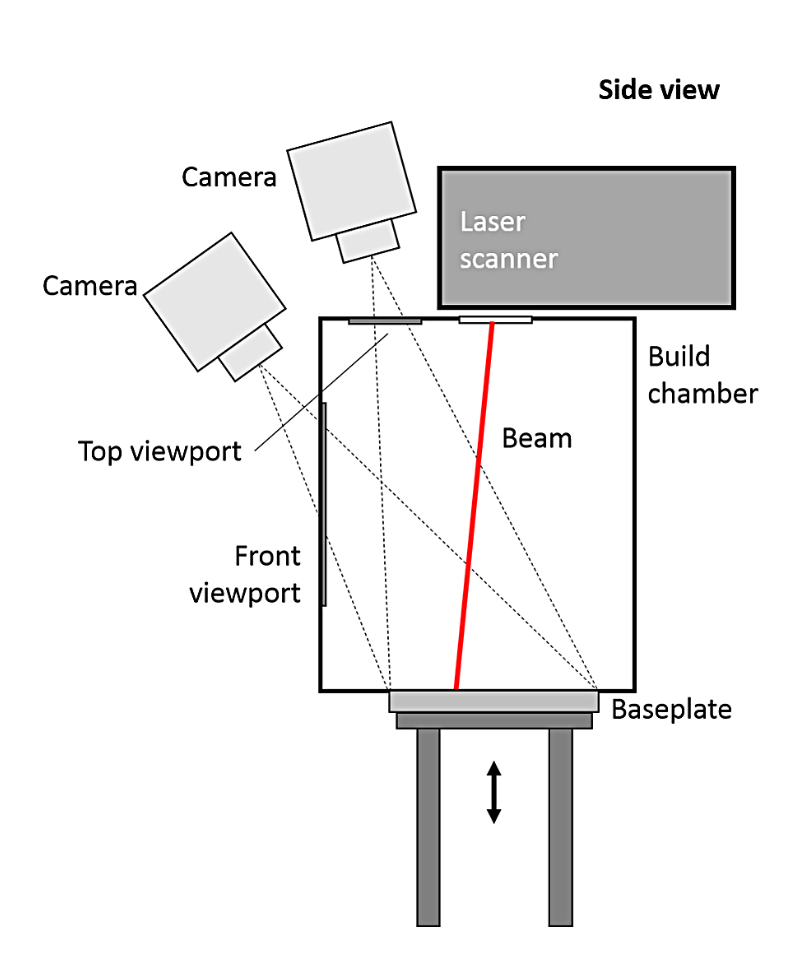
\includegraphics[scale=0.35]{Images/off axial laser.png}
    }
    \qquad
    \subfloat[\label{fig:fig:offaxialebm}]{
        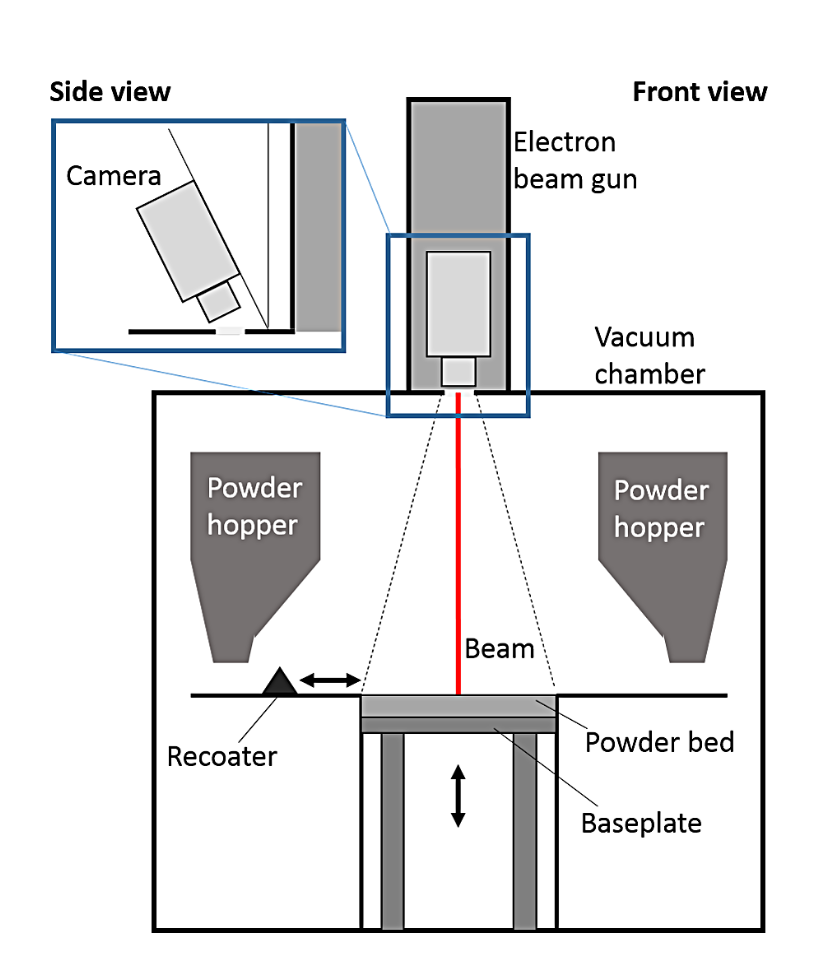
\includegraphics[scale=0.35]{Images/off axial EBM.png}
    }
    \caption[Off-axis sensing.]{Example of off-axis sensing architectures in SLS (a) and EBM (b) \cite{leach_-machine_2020}.}
\end{figure}
In \emph{level ~1}, i.e. measurement and characterisation of layer properties, we can distinguish two further types of measurements. The first is conducted before laser scanning, which allows us to identify areas where the powder is not uniform, potential defects produced by the recoating system or super-elevated edges. The second is performed after the laser scanning, through which we can detect any contamination of the powder of the printed slice or any geometric or dimensional deviations from the nominal shape. There are several types of sensors that can be employed for anomaly detection at this level.
\begin{figure}
    \centering
    \subfloat[\label{fig:quadratoir}]{
        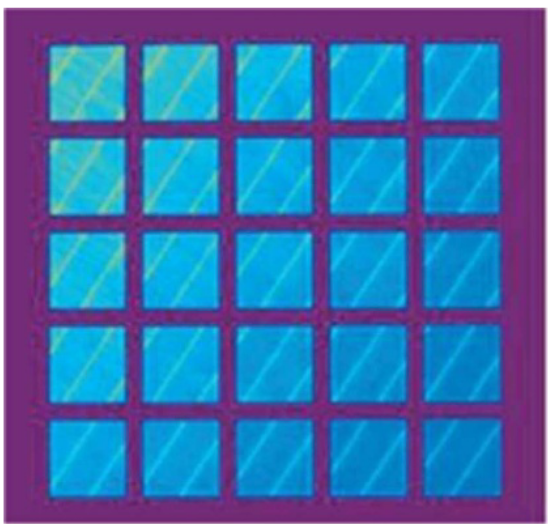
\includegraphics[scale=0.45]{Images/quadratoir.png}
    }
    \qquad
    \subfloat[\label{fig:cilindroir}]{
        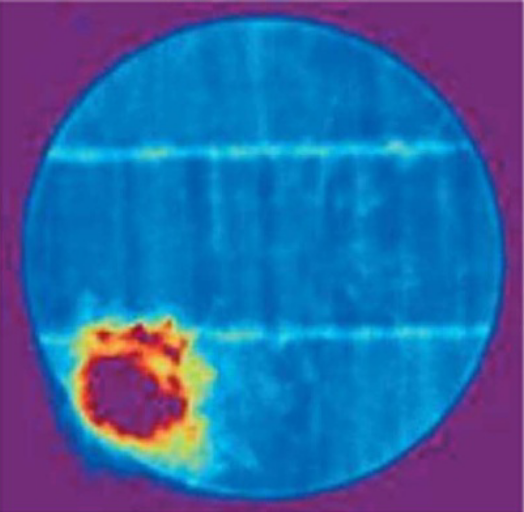
\includegraphics[scale=0.45]{Images/cilindroir.png}
    }
    \caption[Optical tomography examples.]{Examples of optical tomography images for cubic samples with variation of energy density (a) and a cylinder produced under shielding gas flow variation (b)\cite{bamberg_-process_2016}.}
\end{figure}
\paragraph{Off-Axis Sensing.} In both SLS and EBM, off-axis sensing is suitable to gather information. Conventional camera operating in the visible range are usually employed in L-PBF (Fig. \ref{fig:offaxiallaser}), while the high temperatures in EBM recoating and the difficulty to install additional sensors on EB-PBF machines (Fig. \ref{fig:fig:offaxialebm}), makes their usage more challenging. The off-axis optical camera within the visible range, however, has a significant drawback: numerous publications as \citealt{kleszczynski_error_2012} (2012) and \citeauthor{foster_bk_optical_2015} (2015) have shown how appropriate illumination condition greatly impacts the camera's acquired result. Both the surface pattern of the printed slice and the powder bed, as well as the contrast between the background (powder) and foreground (printed slice) areas, are influenced by the intensity, nature, and relative angle of the illumination source. Hence, non-uniform illumination conditions may mask some anomalies and it involves some post-acquisition operations that might be challenging. The relative angle between the camera and the illumination source also plays a relevant role in this kind of measurement as shown in  \citeauthor{caltanissetta_characterization_2018} (2018). Moreover, the distorted perspective given by the camera's positioning needs to be corrected through specific geometric adjustment operations before analysis. In addition to traditional cameras, those operating in the NIR/IR range can also be used in process monitoring of level 1 process signatures. They are particularly suitable in EBM processes due to the high temperatures encountered during the printing process. Two examples of acquired images can be seen in Fig. \ref{fig:quadratoir} and Fig. \ref{fig:cilindroir}. One of the most employed system for this kind of measurement is ‘LayerQam’, developed by Arcam (GE Additive) for integration in its EB-PBF machines. The system consists of a NIR camera that acquires an image of the layer after the melting phase and use local pixel intensity variations to detect anomalies. Furthermore, the presence of bright spots are used as proxies of possible volumetric flaws and material discontinuity defects.
\paragraph{Fringe Projection.} The off-axis imaging techniques mentioned in the preceding paragraph can be used for generating a 2D reconstruction of the powder bed and the printed section. With fringe projection, we can achieve a height map of the powder bed, a 3d representation of the powder. To achieve this map, we need merge of visualization layer with topographic examination. The standard configuration for such measurements consists of a camera (single view configuration) and a projector. The graphic representation of the system can be seen in Fig. \ref{fig:fringesetup}, while in Fig. \ref{fig:fringeprojection} there is an example of an height map.
\begin{figure}
    \centering
    \subfloat[\label{fig:fringesetup}]{
        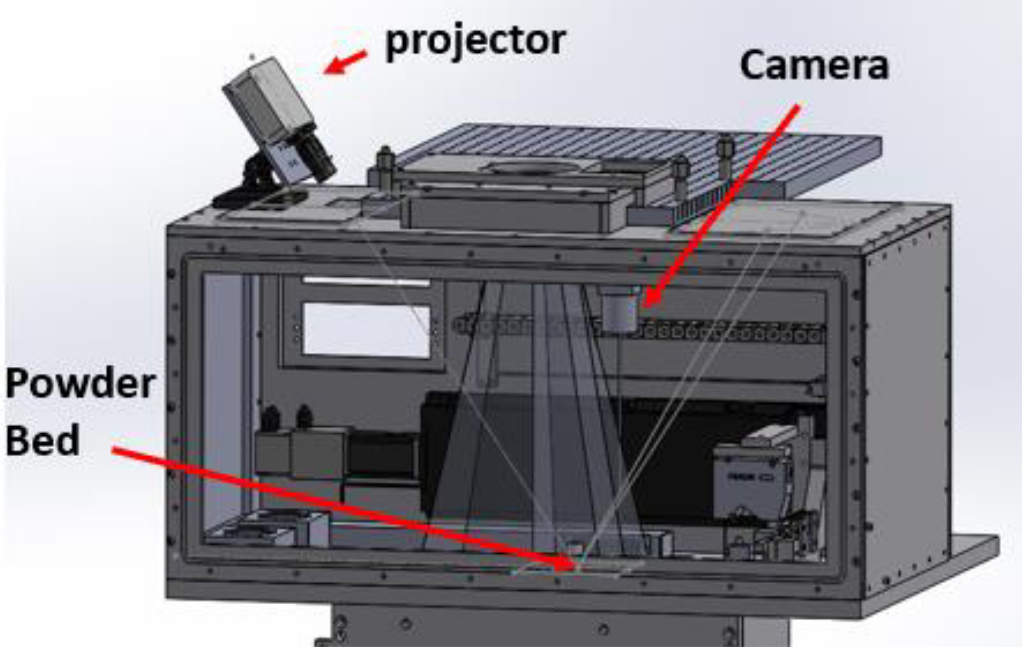
\includegraphics[scale=0.35]{Images/fringesetup.png}
    }
    \qquad
    \subfloat[\label{fig:fringeprojection}]{
        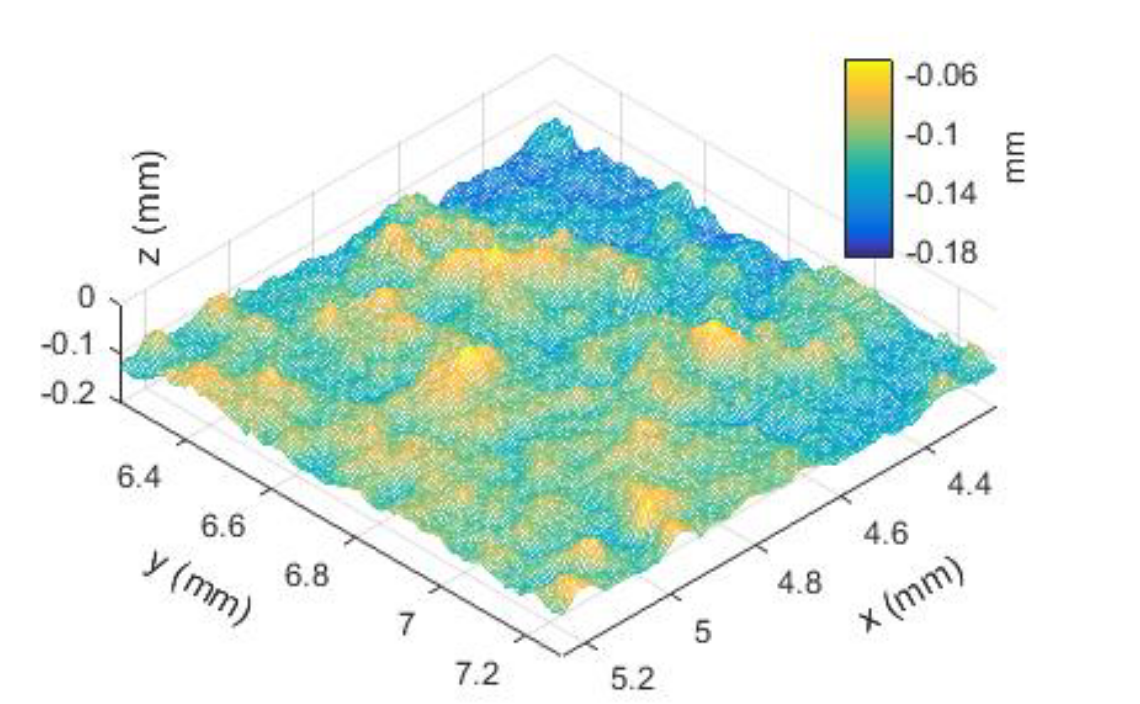
\includegraphics[scale=0.35]{Images/fringeprojection.png}
    }
    \caption[Fringe projection.]{Setup for fringe projection measurement system (a) and reconstructed height map of the power bed (b) \cite{zhang_situ_2016}.}
\end{figure}
Other authors proposed and tested multi-view configurations, with two or more cameras, suitable to achieve higher resolution and accuracy, like in \citeauthor{kalms_new_2019} (2019).
\paragraph{Blade Mounted Sensor.} Another possible approach for level 1 process monitoring is to employ an optical sensor directly mounted on the recoating blade of PBF printers. In this way, we can avoid the geometric distortion typical of off-axis systems. Moreover, these sensors can be used both for obtaining a 2D representation of the print bed and for reconstructing the height maps. In the former case, we can obtain a resolution up to \SI{4800}{DPI} over a length of \SI{210}{\milli\metre} with a spatial resolution of \SI{5.3}{\micro\metre / pixel} \cite{tan_phuc_high-resolution_2019}, while in the latter with a little lower resolution of \SI{20}{\micro\metre / pixel} \cite{barrett_micron-level_2018}.
\paragraph{Co-axial sensing.} L-PBF offers the possibility to leverage the back-scattered light from the melt pool and its adjacent areas, to gauge specific metrics indicative of melt-pool dynamics. Scattered light pass through the optical path of the laser, passing the same lenses of processing laser, and a semi-reflective mirror redirects the laser beam to the scanner, while simultaneously allowing the light emitted from the melt pool to be detected by sensors. This emitted light is then divided and directed to each sensor. Various co-axial detection designs might encompass multiple pyrometers, bi-wavelength or multi-wavelength pyrometers, and assorted imaging devices in either the visible or infrared spectrum. An example of a co-axial sensing system can be seen in Fig. \ref{fig:coaxiallaser}. With this method, we can reach really high sample rates of \SI{50}{\kilo\hertz}, but the observation area is typically limited to \qtyproduct{0.5 x 0.5}{\milli\metre}, making this method unsuitable to capture time evolution. Alterations in the melt pool's dimensions and luminosity/temperature can induce changes in the pyrometer's readings, facilitating the observation of melt pool consistency and any unusual signal shifts. This architecture was first developed by the Katholieke Universiteit Leuven and licensed by Concept Laser \cite{leach_-machine_2020, kruth_jean-pierre_feedback_2007, berumen_quality_2010}. This measurement approach has achieved outstanding results, with a lateral resolution of \SI{30}{\micro\metre} and a vertical resolution of \SI{7}{\micro\metre} \cite{fleming_tracking_2020}.
\begin{figure}
    \centering
    \subfloat[\label{fig:coaxiallaser}]{
        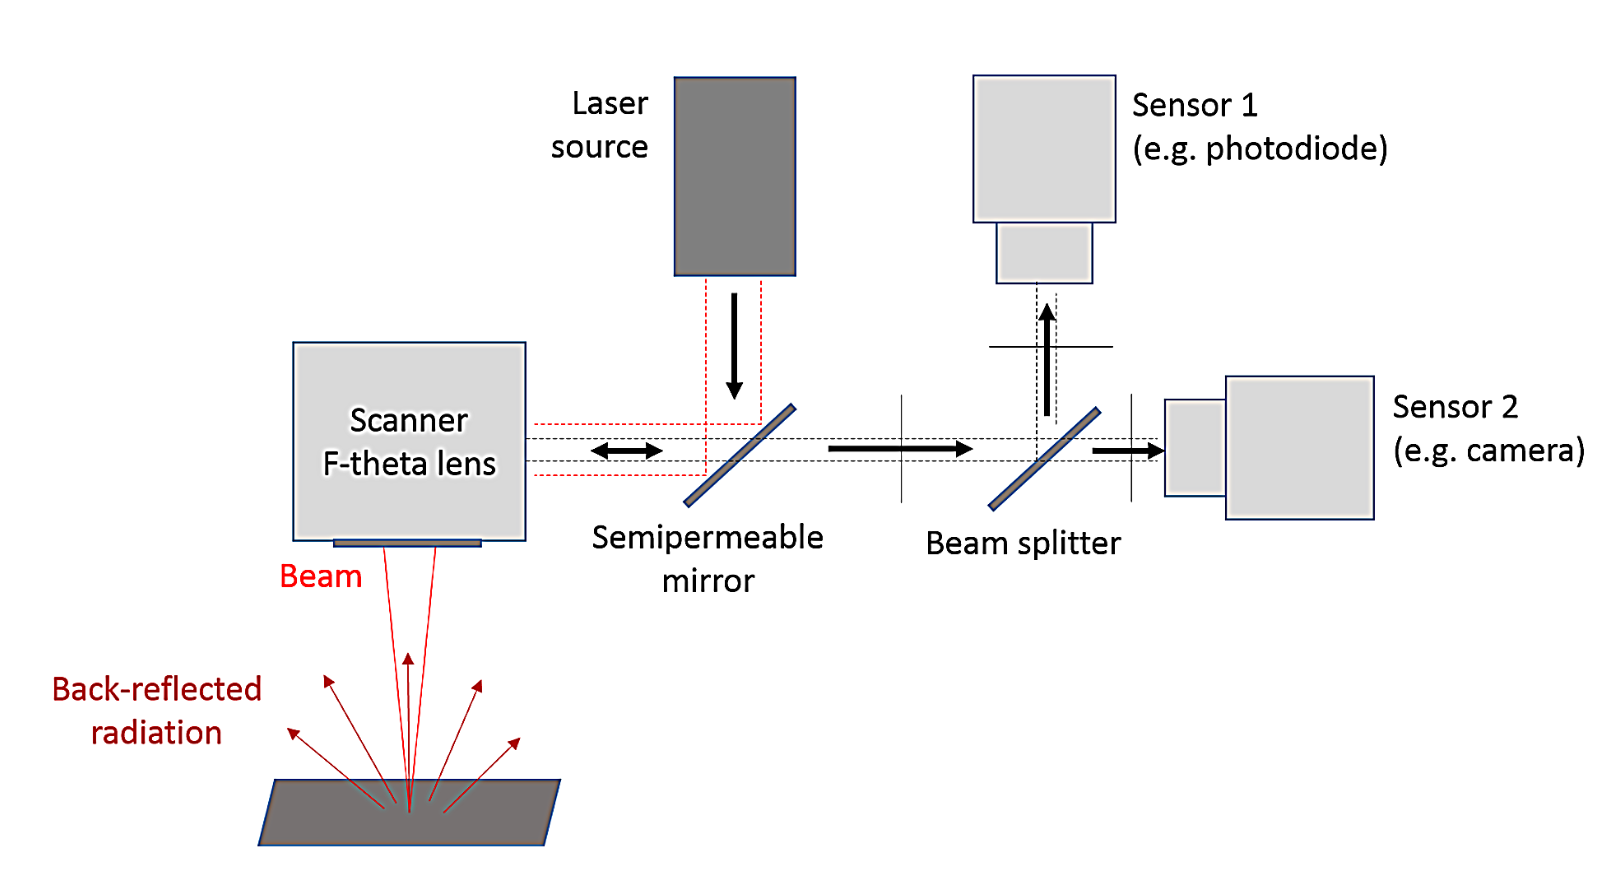
\includegraphics[scale =0.35]{Images/coaxial laser.png}
    }
    \qquad
    \subfloat[\label{fig:coaxialheatmap}]{
        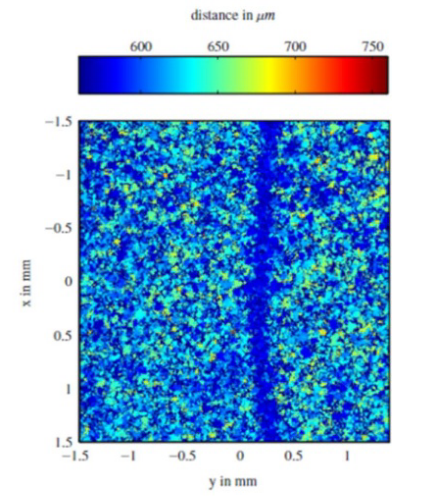
\includegraphics[scale=0.5]{Images/coaxialmap.png}
    }
    \caption[Co-axial sensing and results.]{A graphical representation of a system for co-axial sensing in L-PBF \cite{leach_-machine_2020} (a) and a corresponding in-situ topography reconstruction (b) \cite{neef_low_2014}.}
\end{figure}
\paragraph{Electronic imaging.} In EBM, the process gives rise to by-products like secondary and backscattered electrons, as well as x-rays. The electrons generated from the interaction between the beam and metal powder could be harnessed could be used to produce an electronic representation of the layer. Thus, one of the undesired effects outlined in Section \ref{sssec:electroninteractions} can be levered to extract valuable insights about the current state of the process. Using only back-scattered electrons electrons, \citeauthor{wong_pilot_2019} (2019) were able to reach a spatial resolution of \SI{60}{\micro\metre / pixel} We can see an example in Fig. \ref{fig:electronic1}. Moreover, we can use electron beam to scan the layers and metal surfaces, using the heat shield as an electron collector also during the melting phase as done by \citeauthor{arnold_operando_2020} (2020), thus it is a real-time measurement. This approach lead to a resolution of \numrange[range-phrase=--]{50}{100}\unit{\micro\metre / pixel}. An image from the study can be seen in Fig. \ref{fig:electronic2}.
\begin{figure}
    \centering
    \subfloat[\label{fig:electronic1}]{
        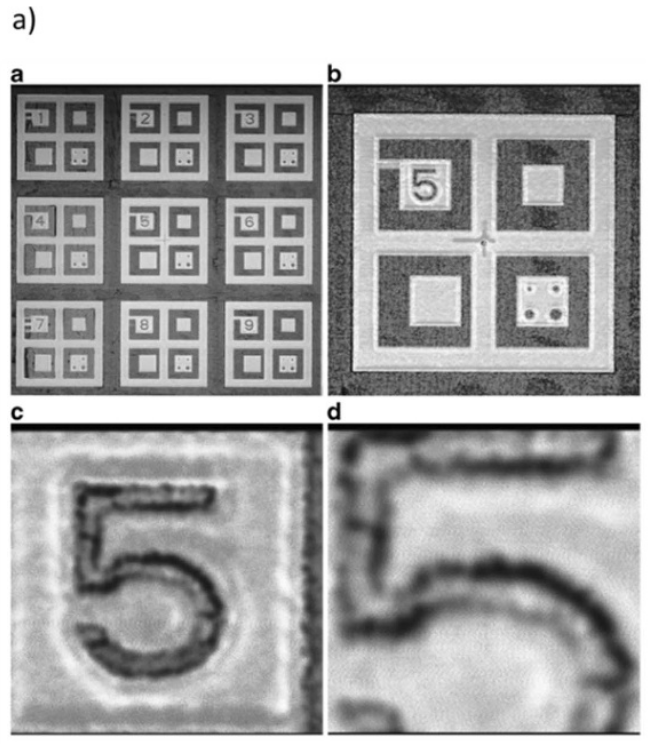
\includegraphics[scale=0.44]{Images/electronic1.png}
    }
    \qquad
    \subfloat[\label{fig:electronic2}]{
        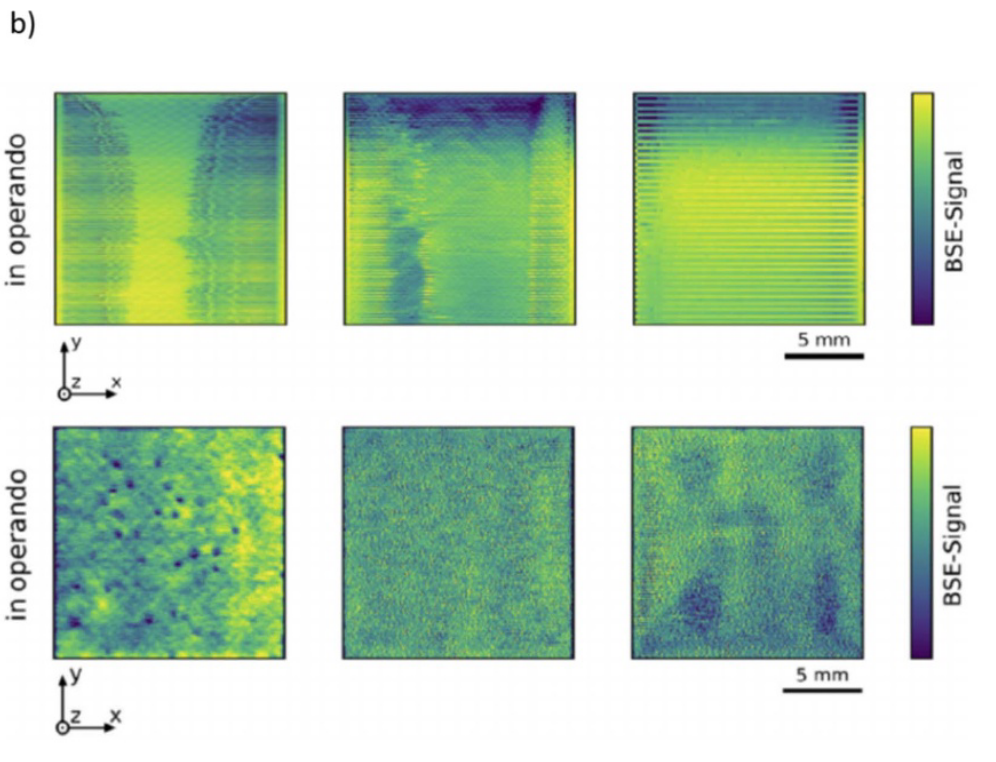
\includegraphics[scale=0.44]{Images/electronic2.png}
    }
    \caption[Co-axial sensing result.]{Examples of electronic images in EBM: images with different magnification factors (a) \cite{wong_pilot_2019} and images of squared printed areas generated via real-time back-scattered signal acquisition from different materials and with increasing hatch spacing \cite{arnold_operando_2020}.}
\end{figure}
For \emph{level ~2} signatures, we use sensors for in-process measurement of fast transient phenomena and high-speed emissions during laser or electron beam scanning. The main goals of this level is to understand underlying physical phenomena which lead to the formation of the defect. Most of the methods used in this level involve off-axis mounted sensors, mainly cameras in the visible range or thermal cameras with really high temporal resolution. Indeed, this is needed to capture fast and transient phenomena. There are different research streams.
\paragraph{Measurement of Process Heatmap and Temperature Profiles.} We will address this paragraph with greater detail as these are the methods used to detect the defects that will be discussed in Section \ref{sec:hotspot}.
\begin{figure}
    \centering
    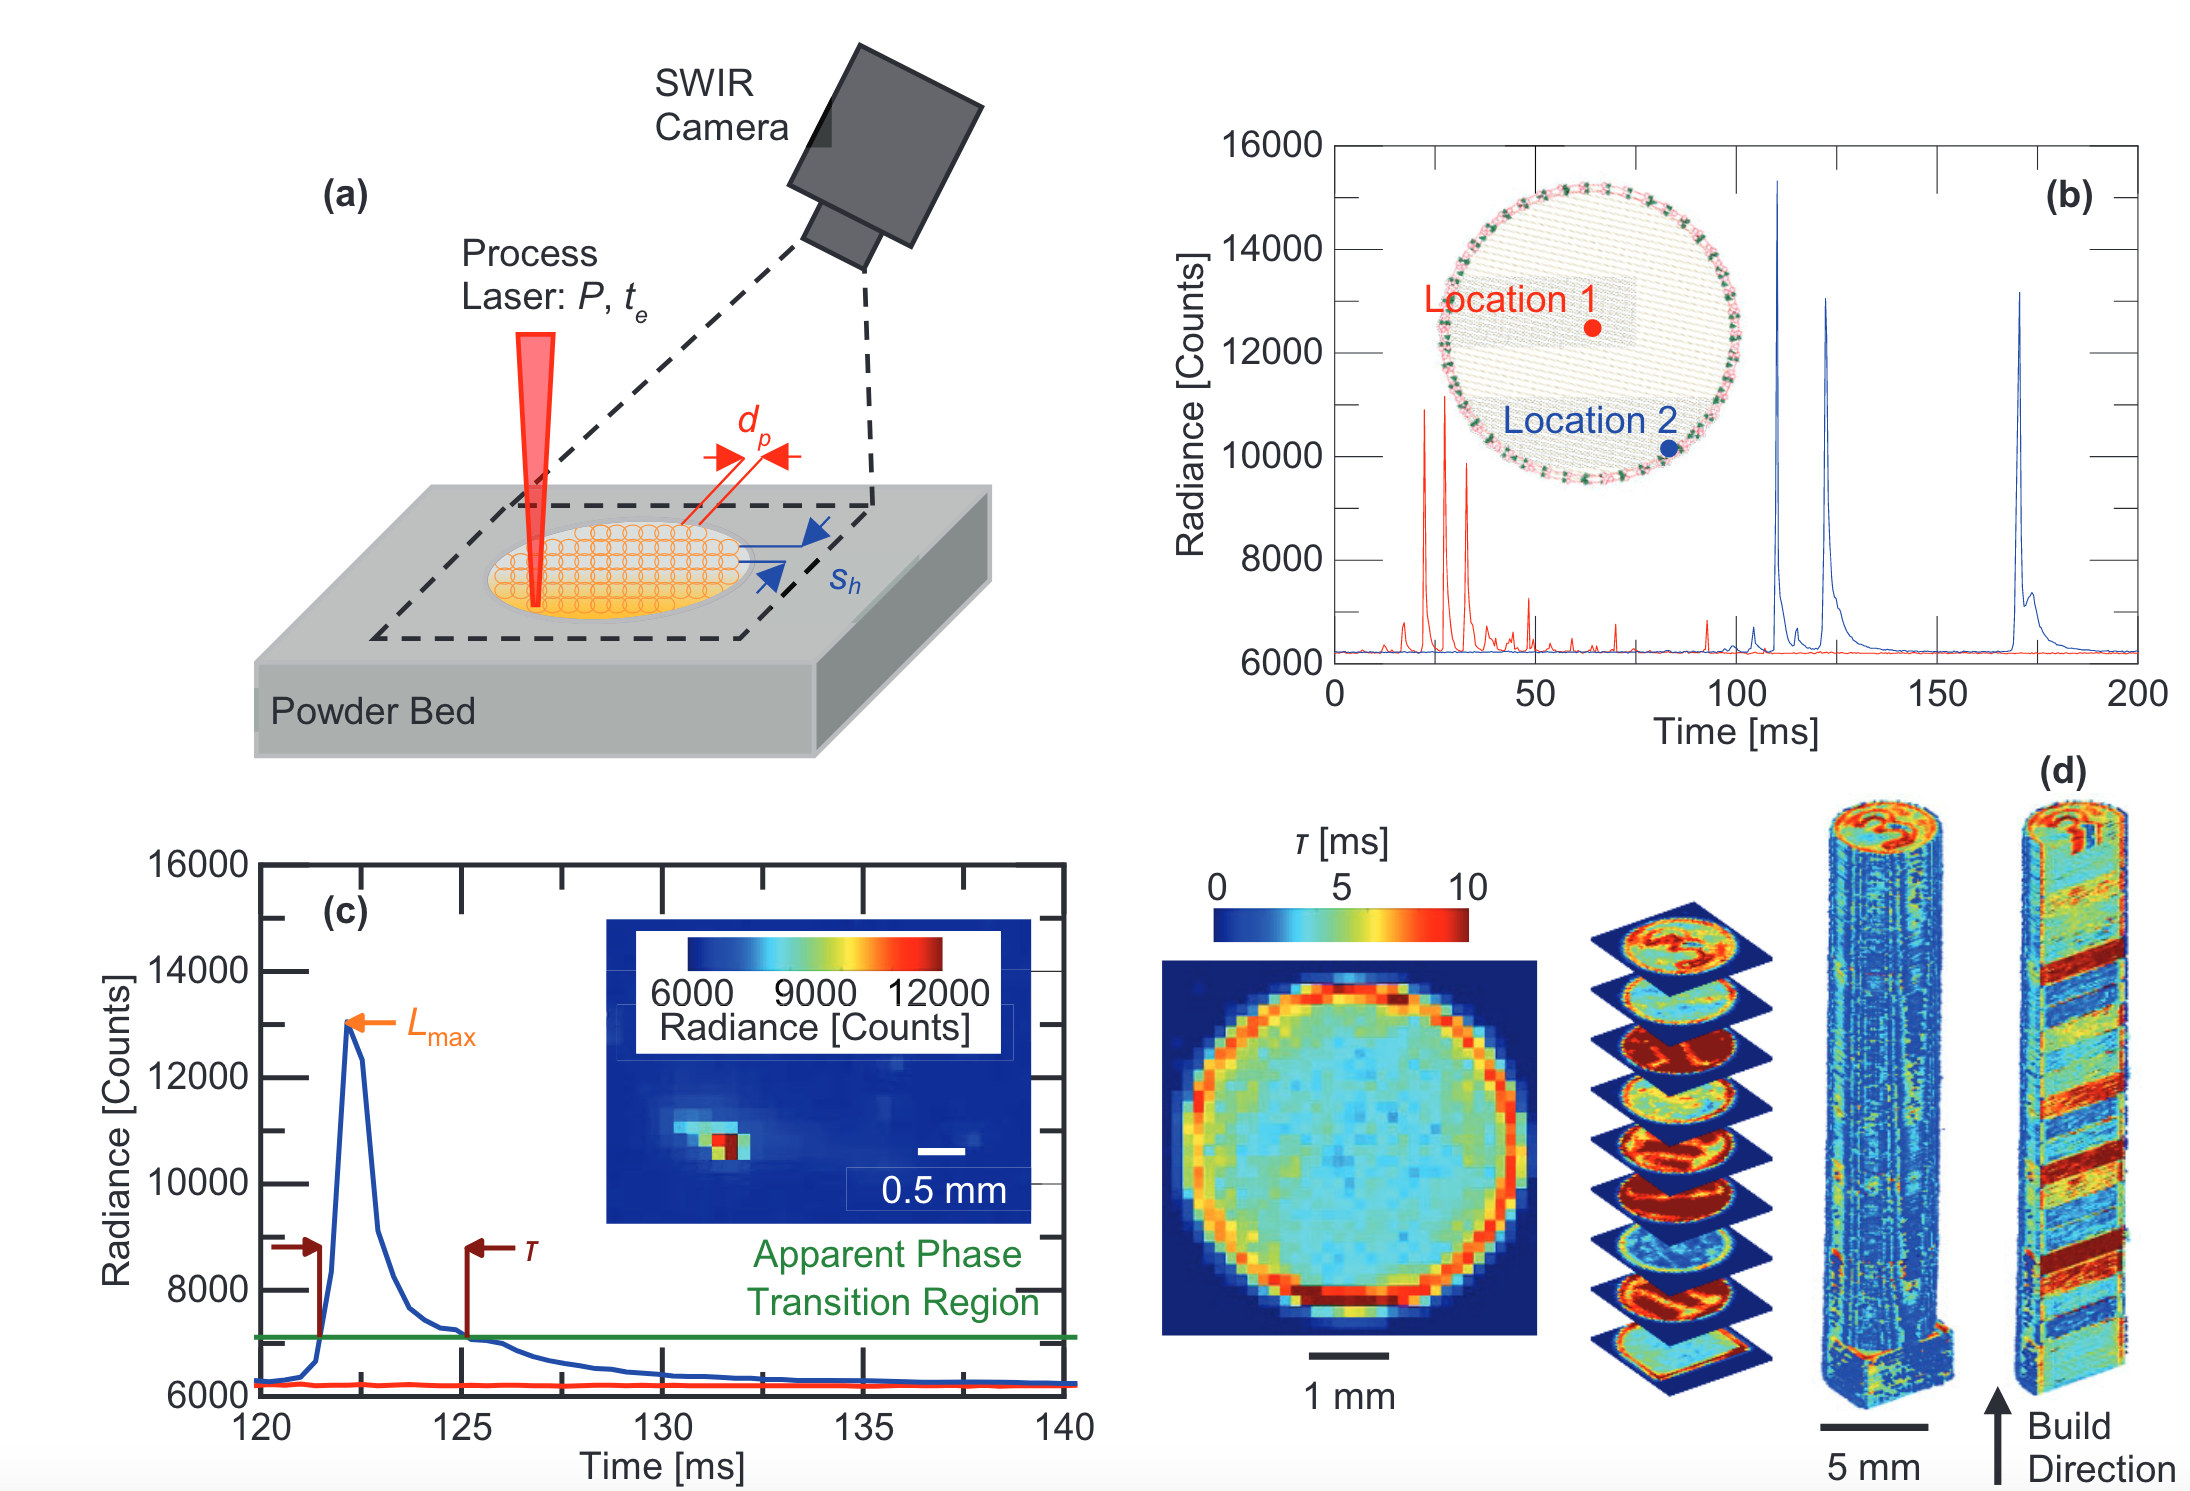
\includegraphics[width=0.8\textwidth]{Images/voxel.png}
    \caption[Example of voxel thermic reconstruction.]{(a) SWIR camera observation of SLM process, (b) time series data from location in center of part cross-section (location 1) and border scan region (location 2), (c) definition of thermal features in time series data with melt pool image, and (d) thermal feature maps showing generation of volumetric data and slicing \cite{lough_-situ_2019}.}
    \label{fig:voxel}
\end{figure}
The layerwise manufacturing paradigm allows the "seeing" of the thermal history of the process, in a new dual-paradigm. In this new paradigm, time and space overlaps over the z-axis. Indeed, the production of an object using additive manufacturing grows in the same direction over time and space. \citeauthor{williams_situ_2019} (2019) demonstred that almost all major quality characteristics of the final part and its mechanical performance depend on the thermal history. Local and global variations of heating and cooling patterns may have effects on material solidification at volumetric, microstructural and geometrical levels. We can identify two primary goals linked to this monitoring systems. The first focuses on building a heatmap of the layer using data collected at slower rates (up to 50 fps), and the other targets recording rapid thermal fluctuations, with time resolutions ranging from \numrange{300}{10000} \unit{fps}. In term of spatial resolution, we can use measurement setups with a limited field of view, which enable us to reach a resolution of \numrange[range-phrase=--]{8}{100}\unit{\micro\metre / pixel}, or with a field of view covering the entire build area, with a resolution typically above \SI{100}{\micro\metre / pixel}. In both L-PBF and EBM we can use thermal cameras, either in the short, medium or long wave IR. To minimize measurement errors caused by the laser's light emissions, we should use a short wave IR camera, with a band-width from \numrange{1.35}{1.6}\unit{\micro\metre} \cite{heigel_situ_2020}. \citeauthor{lough_-situ_2019} (2019) using this type of camera, they were able to produce a thermal map of a specimen printed with L-PBF. Then, using extracted features from the map, they achieved a voxel-based representation of the part, associated with its local and global quality attributes. In Fig. \ref{fig:voxel} there is the reconstruction of the specimen. Other researchers have employed high temporal resolution IR video imaging in L-PBF to improve the ability to map temperature profiles spatially and temporally, also capturing quick and transient events. Although they exhibit an high sensitivity to emissivity values when determining absolute temperatures, thermal cameras in the medium or long wave IR spectrum can be adjusted over a broader temperature span compared to short wave IR cameras. They maintain high sensitivity even at elevated temperatures, which make them particulary suitable for in-situ thermal video imaging in EB-PBF applications, especially when we need a larger field of view to construct thermal map. In EB-PBF, the methodologies for in-situ video imaging have to be tailored to cater to the unique aspects of the process. Both standard and thermal imaging devices must be shielded against x-ray emissions and metal deposition. To protect sensors we can use x-ray shielding glass and a rotating Kapton film, ensuring that metallic vapours don't settle on the glass. The Kapton film allows for approximately 79\% IR transmission, while a \SI{10}{\milli\metre} x-ray shielding window lets through around 1.08\% of IR, as noted by \citeauthor{ralph_b_dinwiddie_thermographic_2013} (2013). However, PBF processes experience rapid state changes, transitioning from powder to a liquid state and then to a solidified form. This, combined with ongoing alterations in surface attributes and vaporized material emissions, and this could affect accurate estimation of temperature measurements. Luckily, for most of the times, we are interested more in the thermal signature fluctuation over time rather than pinpointing an absolute temperature. In these cases, data analysis and monitoring algorithms can be employed directly on original signals. On the other hand, if we need a precise temperature value, we can use more advanced thermal camera, even if they are big, costly, and generally call for alterations in machinery hardware and viewports for assimilation into working setups. Standard cameras are more cost-effective and straightforward to incorporate and with the right equipment, they can offer high temporal precision. Even though they don't grant precise temperature assessments, variations in pixel brightness in the visible spectrum can be use as proxy to measure thermal shifts to spot abnormalities and imperfections. A rising stream of research consists on identifying localized intense heat events, referred to as 'hot-spots' (HS), using rapid video imaging in the visible domain. A hot-spot is characterized by a localized excessive heating of the layer due to unregulated thermal interactions with the nearby matter.
\paragraph{Process By-Products Measurement.} Due to the different nature of the interactions in the SLS and EBM processes, as already described in \ref{sec:matterint}, we need to distinguish between the measurement systems of the by-products of these two processes. Since we have already discussed the measurement of the by-products of EBM in level 1, in this paragraph we will focus on L-PBF processes. It has been widely demonstrated that the partial vaporization of the metal, also called plume, and the spatter ejected together with it are correlated with detrimental effects on part quality. Indeed, intense emissions of these by-products could lead to the deflection and partial absorption of the laser beam, resulting in a change in the laser spot geometry or energy density. Fig. \ref{fig:plume} shows a graphical representation of the phenomenon just described. To obtain information about spatter and plume, visible and IR video imaging techniques can be employed. In Fig. \ref{fig:colosimoplume} we can see an example of an in-control plume generation phenomenon acquired using IR camera. Recent research has introduced a high-speed stereo vision system to identify and trace individual spatters in the 3D space above the layer. Through this approach, it's possible to monitor the trajectory of spatters, allowing for the calculation of both their speed and their spatial-temporal behaviours. Tracking the spatter along its course can enhance the understanding of process byproducts, offering further clarity regarding their formations and the effect of processing conditions. To be able to track the spatter's origination mechanism we can use an high-speed, high-energy x-ray video imaging system.
\begin{figure}
    \centering
    \subfloat[\label{fig:plume}]{
    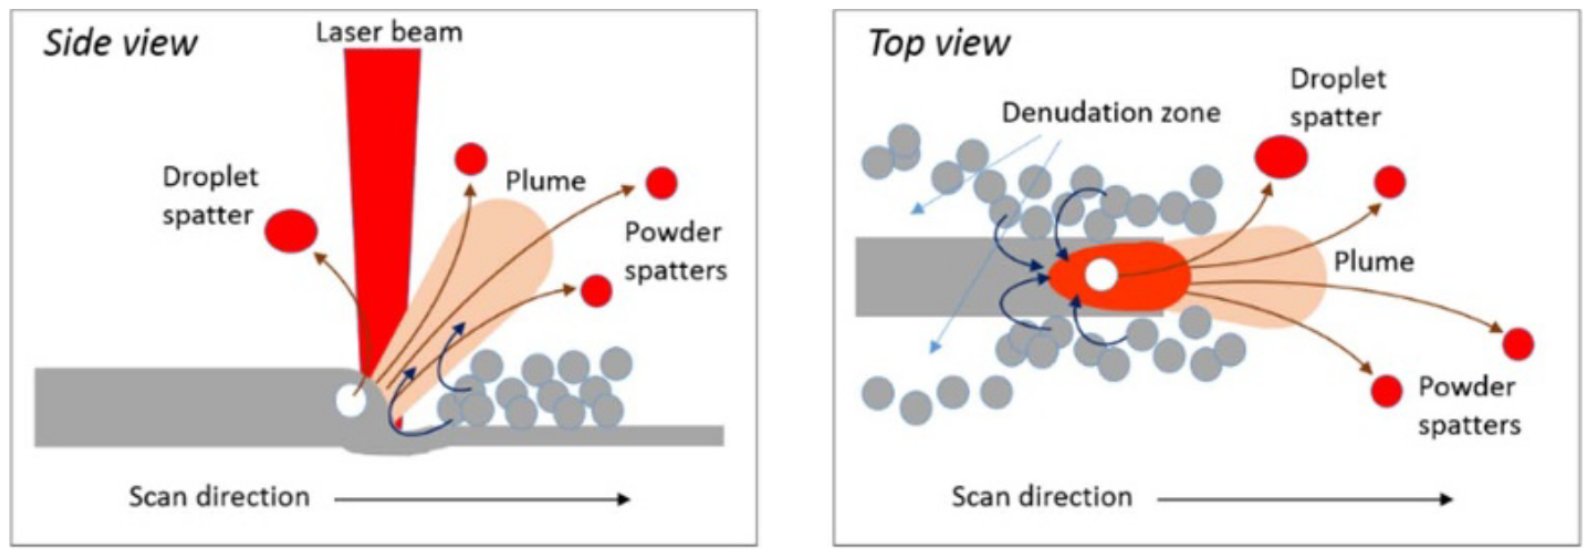
\includegraphics[scale = 0.4]{Images/plume.png}}
    \qquad
    \subfloat[\label{fig:colosimoplume}]{
        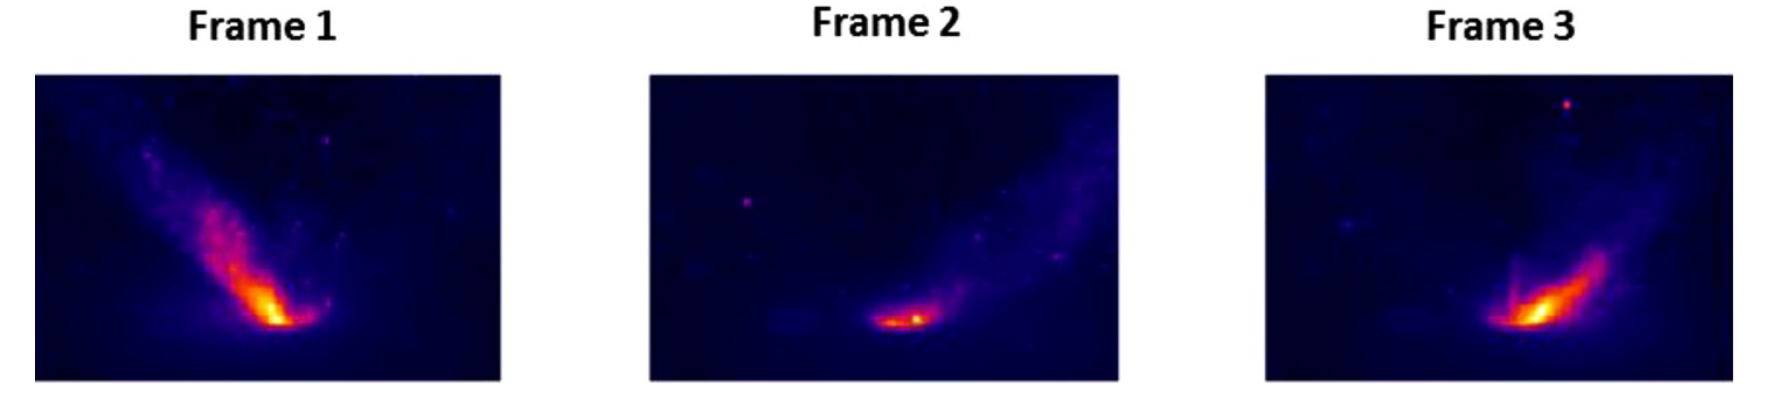
\includegraphics[scale=0.4]{Images/plumecolosimo.png}
    }
    \caption[Spatters and plume in SLS]{Schematic representation of spatters and plume emission in SLS (a) \cite{grasso_-situ_2021}, and plume emissions captured with long wave IR video imaging (b) \cite{grasso_statistical_2019}.}
    
\end{figure}

\begin{figure}
    \centering
    \label{fig:barretspatter}
    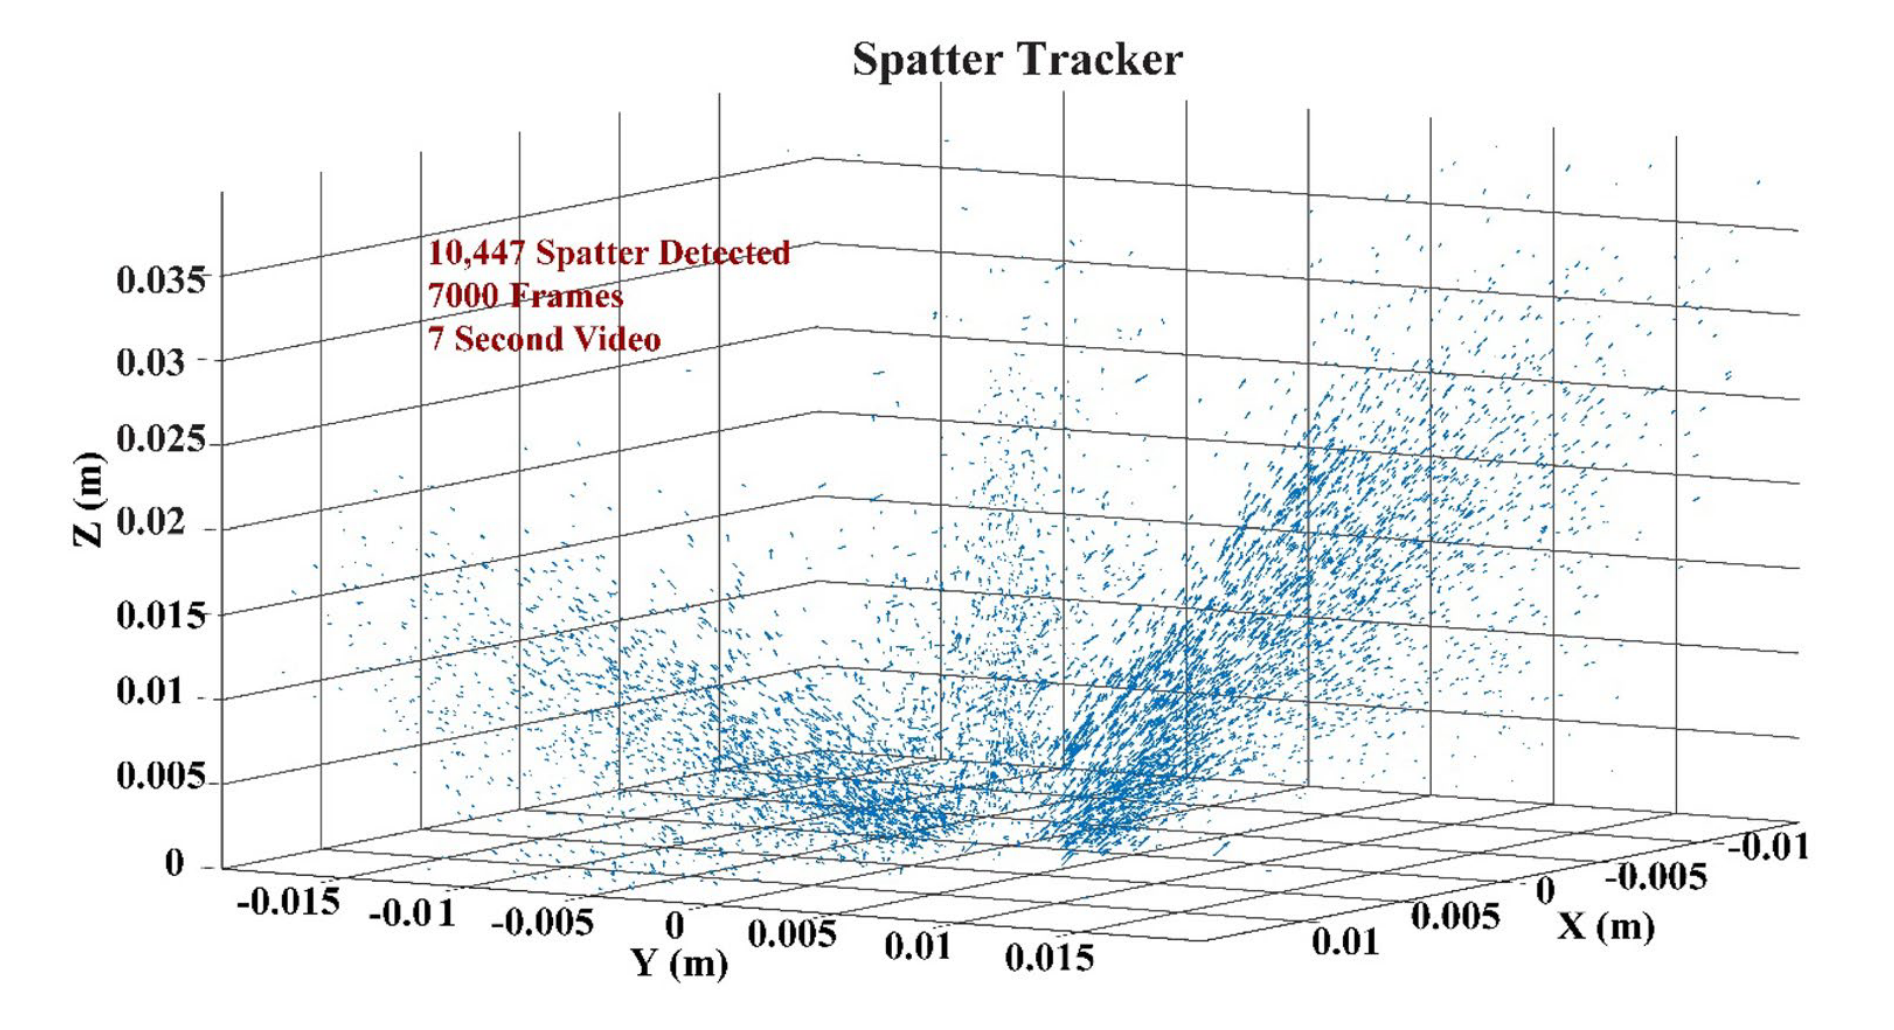
\includegraphics[scale=0.3]{Images/splatter.png}
    \caption[3D spatter reconstruction.]{Reconstructed of 3D spatter localisation via high-speed stereo vision (b) \cite{barrett_statistical_2019}.}
\end{figure}

\paragraph{Measurement of air-borne acoustic emission.} In L-PBF processes, there is a research streams that involves airborne acoustic emission sensors. The measurement system consists of capturing air density variations during the laser scanning by placing the sensor in the proximity of melted area. To measure acoustic vibration, we can use Bragg grating opto-acoustic sensor installed into the build chamber at about \SI{200}{\milli\metre} from the process zone, with a sampling frequency of \SI{1}{\mega\hertz}. In \citeauthor{wasmer_situ_2019} (2019), the sensor was placed so that the longitudinal axis of the fibre was perpendicular to the acoustic wave to increase its sensitivity. The result of the study can be seen in Fig. \ref{fig:acustic}. We can appreciate how different level of porosities correspond to different level audio waves. We can also use more common sensors like in \citeauthor{ye_defect_2018} (2018). In the study, authors installed a microphone into the build chamber at an angle of \ang{30} above the build area, with a frequency response in the range \numrange[range-phrase=--]{0}{100}\unit{\kilo\hertz}. The resulting measurements and their information content in the temporal and/or frequency domain can be viewed as signatures of the laser-material interaction.
The melt pool carries a lot of information since it is the phenomenon with the highest granularity possible in PBF. Monitoring the properties of the melt pool are processes involved in \emph{level 3}. These systems have primarily been explored in L-PBF, since co-axial sensors can be easily employed. Indeed, co-axial sensing is prevalently employed at this level. We have already discussed some level 2 methods in EBM to extract details at both the track and melt pool levels using off-axis video imaging. Recently, there's been emerging research focused on analyzing melt pool data using machine learning methods. We can identify two primary measurement systems: methods that integrate over space and those that resolve spatial details.
\begin{figure}
    \centering
    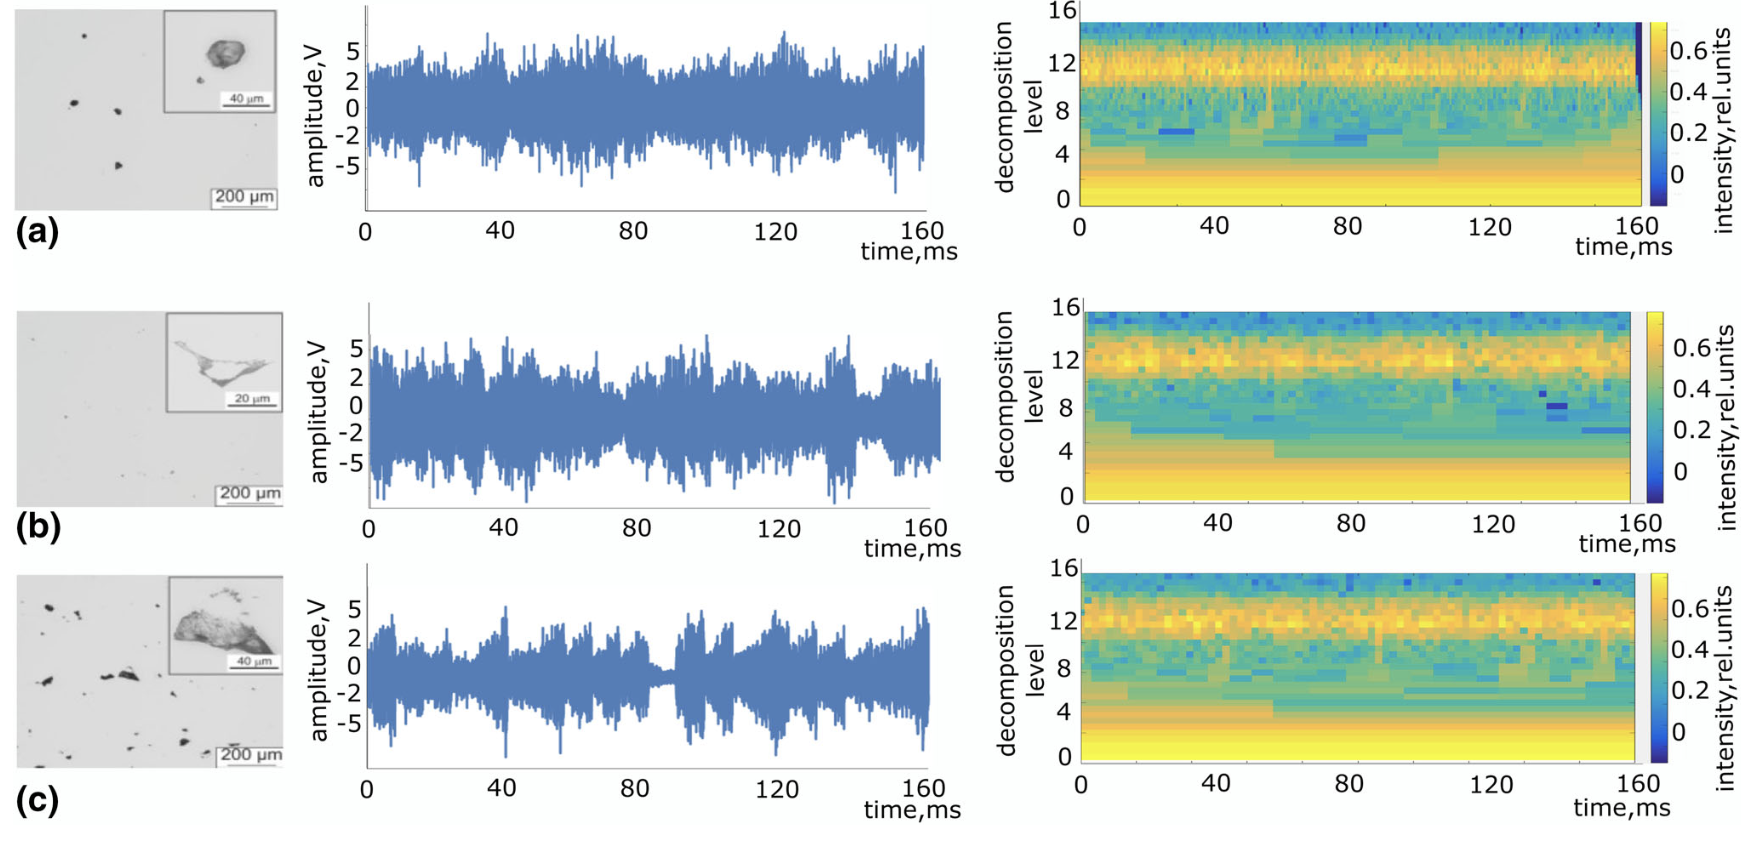
\includegraphics[width = 0.8\textwidth]{Images/acustic.png}
    \caption[Example of AE of different porosities specimens.] {From left to right, typical light microscope cross-sectional images with different porosities, their corresponding acoustic emission signals with a \SI{160}{\milli\second} time span, and their corresponding wavelet spectrogram of the regions produced with different scanned velocity \SI{300}{\milli\metre / \second} (a), \SI{500}{\milli\metre / \second} (b) and \SI{800}{\milli\metre /\second} (c) \cite{wasmer_situ_2019}}
    \label{fig:acustic}
\end{figure}
\paragraph{Spatially integrated methods.} Real-time co-axial monitoring of melt pool attributes has been employed since 2010. At this level, process signatures are the size of the melt pool, its size, its shape, and the intensity and spectrum of emitted radiation. We can use a spatially integrated pyrometry with a  single or multiple photodiodes, to capturing the intensity of radiation from the melt pool with impressive temporal accuracy, typically at a \SI{100}{\kilo\hertz} sampling rate. Significant parameters influencing acquired data quality include the spectral range of measurement and the sensor's field of view. Most sensors work within a range of \numrange{400}{1100} \unit{\nano\metre}, even if it's hard to find sensors for wavelengths beyond \SI{1000}{\nano\metre}. Today, co-axial photodiodes are equipped in the majority of industrial L-PBF setups. In a certain way, they are slowly becoming embedded sensors of level 0. \citeauthor{montazeri_-process_2018} (2018) showed that chemical composition of the material can be determined via melt pool radiation measurement, finding a way for detecting potential powder contaminations by analysing spectral data. \citeauthor{lough_-situ_2020} (2020) achieved similar results using a co-axial optical emission spectroscope to capture the spectral data and infer the chemical composition of vaporized by products. There are also sensors with larger fields of view, up to the entire build area, which enables measuring of radiation emitted by surrounding hot areas too. However, these sensors have a much lower resolution, not even comparable to that of co-axial sensors.
\paragraph{Spatially resolved methods.} More detailed insights into the melt pool's attributes and its consistency over time can be obtained through co-axial video imaging techniques. Commonly, a high-speed camera (\numrange{1000}{50000} \unit{fps}) paired with a narrow-band NIR filter, is utilized to maximize the dynamic range and record the primary melt pool emissions. In some cases, it is also possible to use off-axis video imaging methods, using high-magnification optics combined with a limited field of view. In \citeauthor{lane_measurements_2020} (2020), the authors employed an off-axis high-speed camera paired with a mirror, which facilitated an up-close examination of the melt pool without interfering with laser beam. They were able to achieve a spatial resolution \SI{3}{\micro\metre / pixel}. In the same paper, authors used also a thermal camera for melt pool thermography and achieved a lower resolution of \SI{36}{\micro \metre / pixel}.
\begin{figure}
    \centering
    \subfloat[\label{fig:colorini}]{
        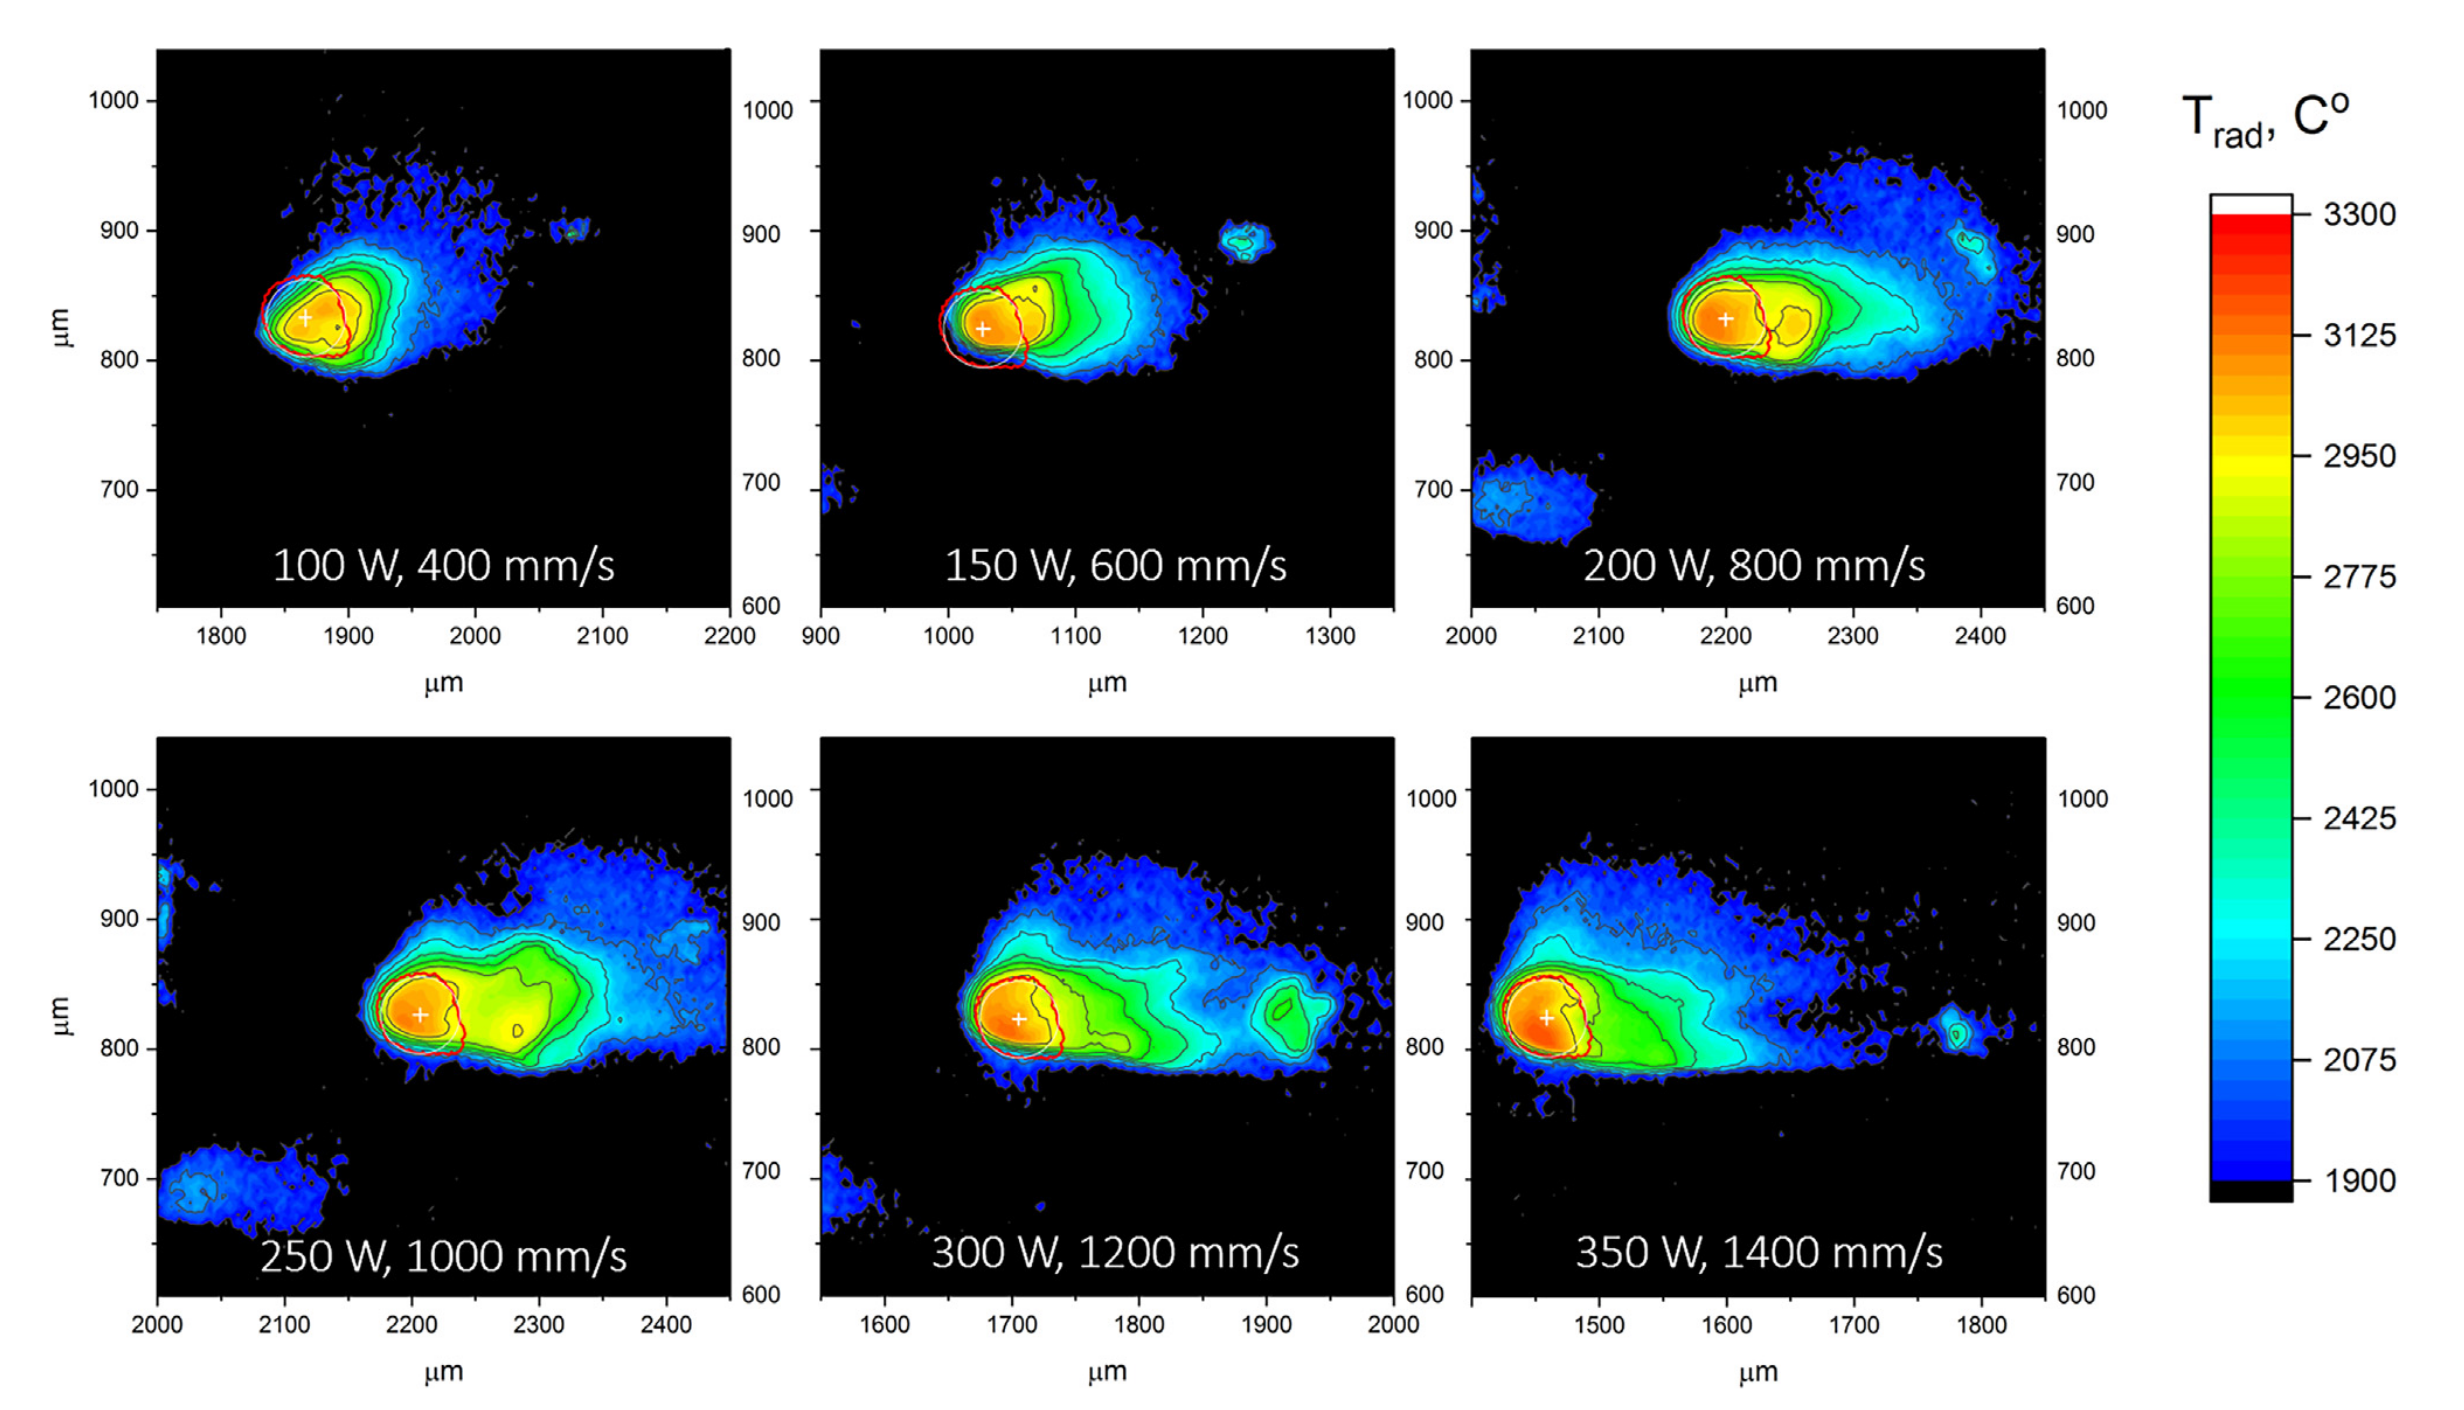
\includegraphics[scale=0.12]{Images/colorini.png}
    }
    \qquad
    \subfloat[\label{fig:spectrograrphy}]{
        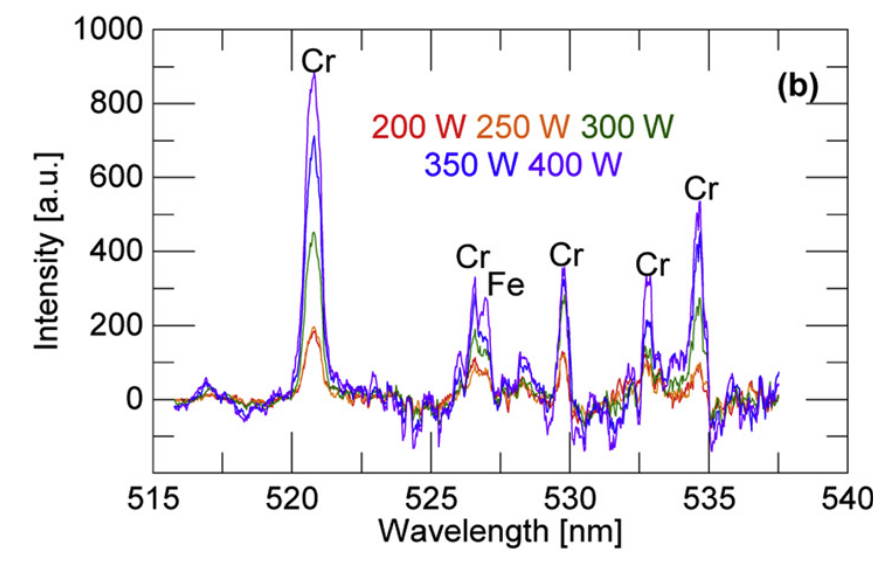
\includegraphics[scale=0.3]{Images/spectrography.png}
    }
    \qquad
    \subfloat[\label{fig:poolthermal}]{
        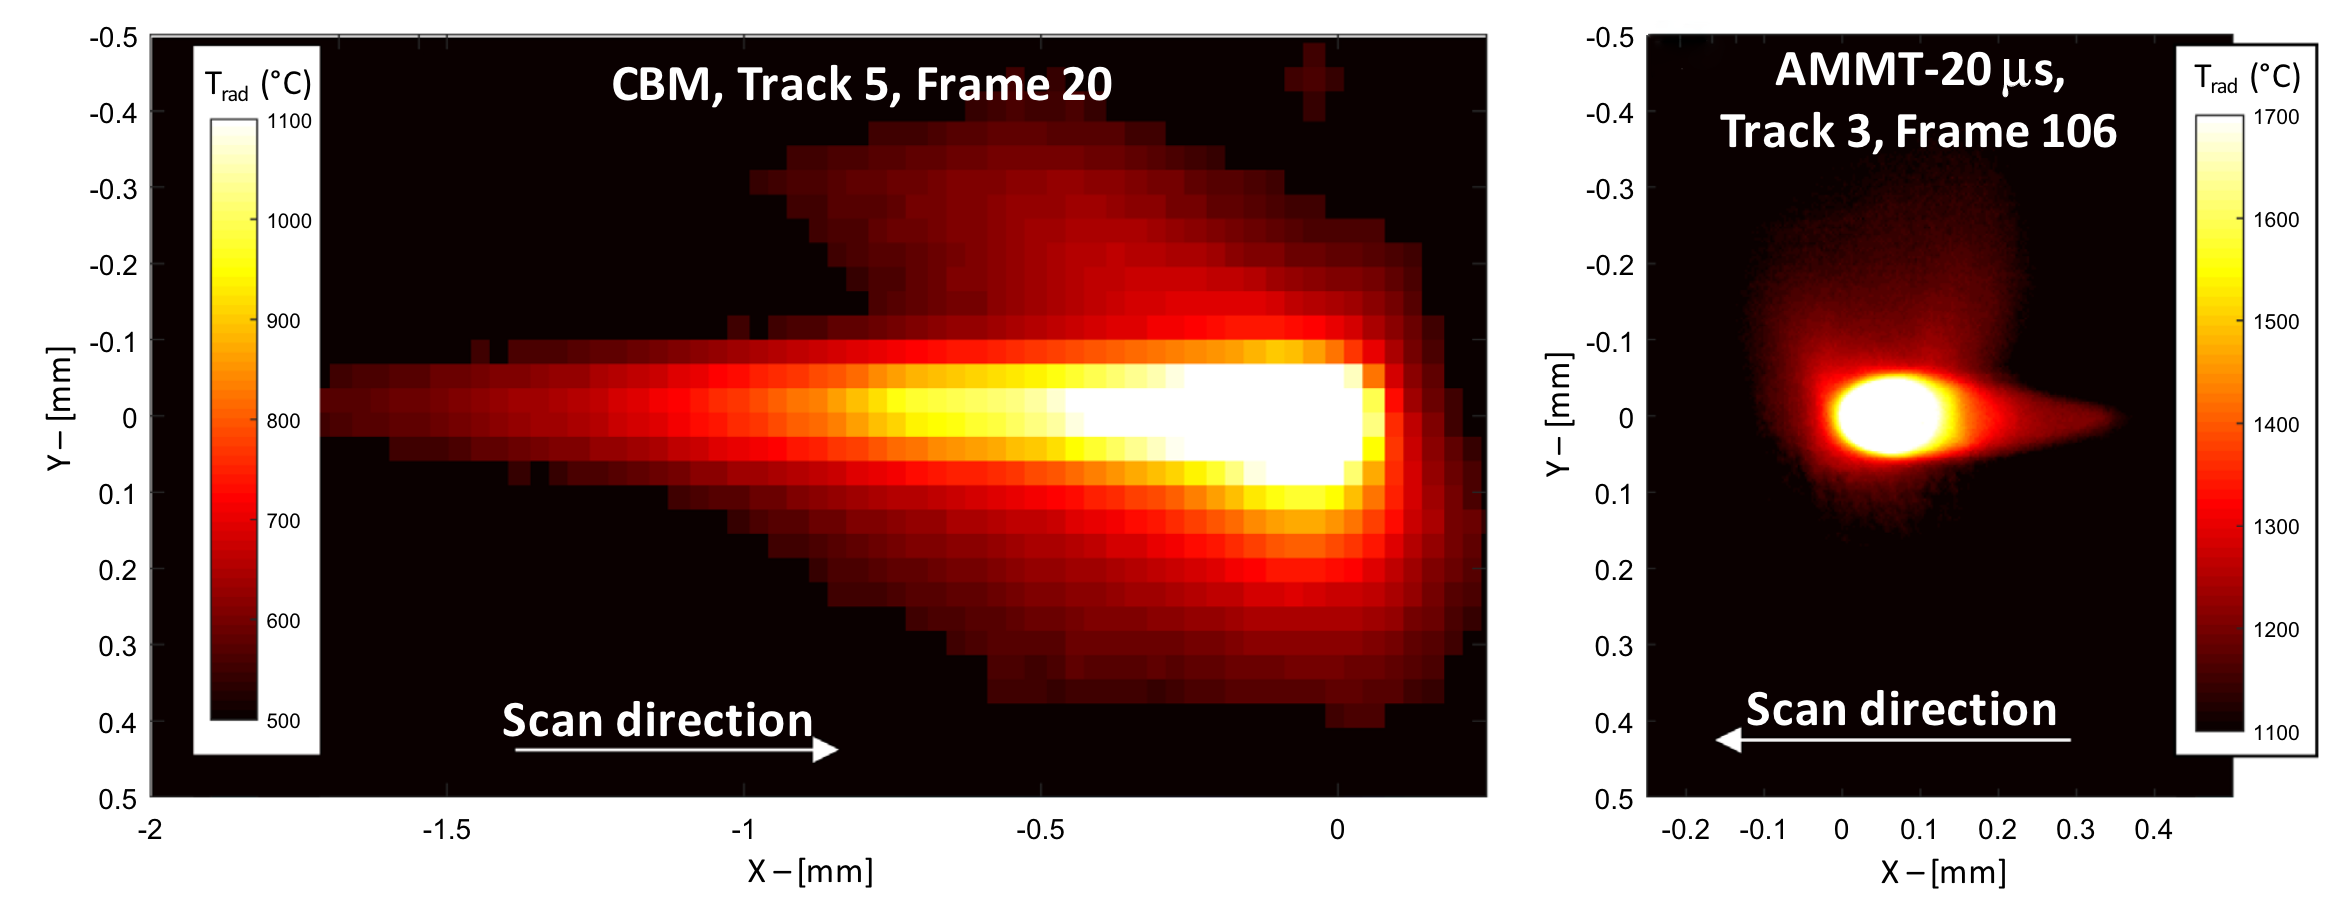
\includegraphics[scale=0.2]{Images/meltpool.png}
    }
    \caption[Level 3 measurement methods.]{Example thermographic video frames aquired using an high speed camera (a) \cite{zhirnov_accurate_2020}, average optical emission spectra of 304L stainless steel (b) \cite{lough_-situ_2020}, and (c) radiance temperature thermal video frames from a thermal camera (left) and high speed camera (right) \cite{lane_measurements_2020}.}
\end{figure}
Another method involves dual-wavelength video imaging, i.e. the acquisition of video sequences at two distinct wavelengths (\SI{700}{\nano\metre} and \SI{950}{\nano\metre}) to enable a temperature estimate via two-colour thermography. This method gets around the problems of guessing the melt pool's brightness by comparing the light levels from the two different wavelengths, thinking they shine consistently at both \cite{williams_situ_2019}.
All the layers discussed so far have one common element: all of them are used for monitoring of the last printed layer, either before, during or after the melting phase. For \emph{level ~4}, the subject of the monitoring process is under the last layer. Indeed, as the layer is being printed, the material characteristics underneath are modified as well, due to partial remelting of adjacent layers and heat exchanges within the build volume. Since it's evident that we cannot use optical devices to monitor what we cannot see, level 4 monitoring relies on other sensors. We ca use high-speed high-energy x-ray imaging systems the gain information about the energy penetration depth and pore formation, or we can use x-ray diffraction measurement to detect any strain and stress formation. Fig. \ref{fig:xray4} shows the result of an x-ray video imaging in L-PBF. Moreover, in last years a new research streams about in-situ x-ray micro-tomography was born. In \citeauthor{lhuissier_situ_2020} (2020), during the in-situ microtomography scan, 1500 projections were acquired resulting in a scan time of \SI{45}{s}, gathering a spatial resolution of \SI{3.64}{\micro\metre / pixel}. Another technique regards the in-situ measurements of acoustic emissions (AEs) and specifically of structure-borne. This technique has also direct application potentials in industry. Structure-borne AEs are suitable to detect sudden releases of elastic energy that propagate within the material, which means that allow us to detect crack formations, detachments of overhang areas from supports or delamination phenomena. We can also use multiple sensors placed at different location in order to triangulate the position of the epicenter of the energy release. A pioneer in the use of AEs in PBF processes is Rieder. In \citeauthor{rieder_-_2016} (2016) he proposed an ultrasonic monitoring device in L-PBF mounted on the underside of the baseplate focusing on the bottom plate interface echo and the backwall echo patterns as proxies of discontinuities in the specimen.
\begin{figure}
    \centering
    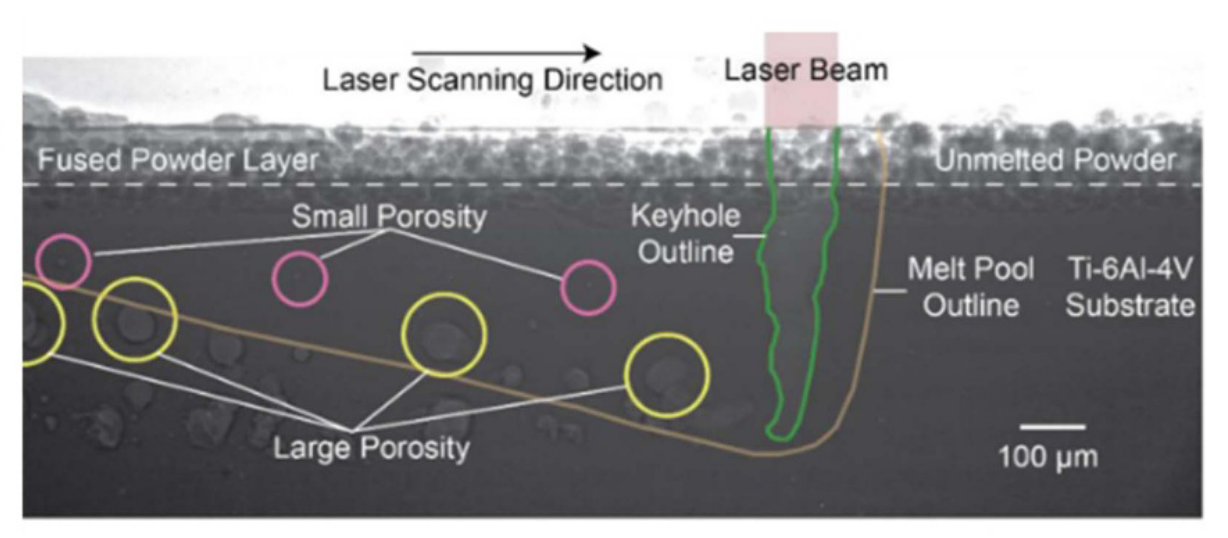
\includegraphics[width=0.65\textwidth]{Images/xray4.png}
    \caption[X-ray video frame.]{Example of an in-situ x-ray video frame with relative defects identified \cite{paulson_correlations_2020}.}
    \label{fig:xray4}
\end{figure}
% <<< End of Sensors for anomalies detection

%%%%%
%%%%%

% Temperature Anomalies and Hot Spots>>>
\section{Temperature Anomalies and Hot Spots}
\label{sec:hotspot}
As discussed in \citeauthor{williams_situ_2019} (2019), almost all major quality characteristics of the final part and its mechanical performance depend on the thermal history. A specific defect characterized by anomalous temperature profiles is known as hot spot (HS). The primary cause of these defects is the laser beam being repeatedly focused on thermally insulated regions. These are areas predominantly surrounded by powder and lacking any support structure to ensure the proper cooling down phase, as explained in Section \ref{sec:pbf_proc}, but also overhanging walls and sharp edges. This would result in a very localized overheating of the powder bed, leading to the following defects \cite{bugatti_towards_2022}:
\begin{itemize}
    \item \textbf{High surface roughness:} overheated areas can lead to melting unwanted areas of powder and partially melted powder particles attach to the surface. This will result into small melted powder on th surface of the final object, thus increasing its roughness;
    \item \textbf{Change in microstructure of the material:} normal melting zone are characterized by a high cooling rate that leads to finer grain formation, while overheating regions tend to develop a coarser microstructure due to the slower cooling transient;
    \item \textbf{Porosity formation:} if the region is already hot, new laser scans may lead to material vaporization, hence unstable keyhole formation which is often correlated with porosity defects.
\end{itemize} An example of these defects can be seen in Fig. \ref{fig:cane}.

\begin{figure}
    \centering
    \subfloat[\label{fig:dio}]{
        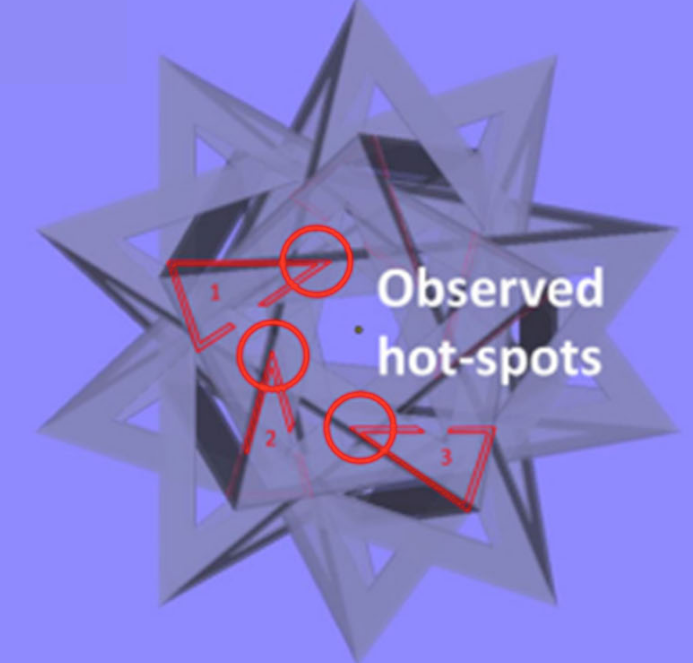
\includegraphics[scale=0.45]{Images/modehs.png}
    }
    \qquad
    \subfloat[\label{fig:cane}]{
        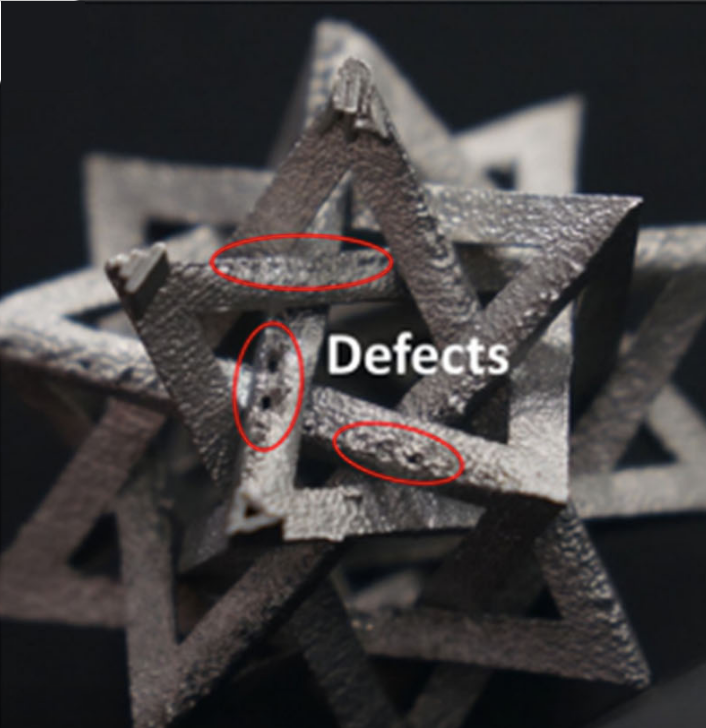
\includegraphics[scale=0.4]{Images/printedhs.png}
    }
    \caption[Examples of hot spot defects.]{Examples of a complex shape CAD model with the position of observed hot spot (a) and relative observed defects in printed part (b) \cite{grasso_-process_2017}.}
\end{figure}
% <<< End of Temperature Anomalies and Hot Spots